\documentclass[11pt]{article}
\usepackage{amssymb,amsmath,amsthm,hyperref,verbatim,pict2e,graphicx,array,listings,appendix,color}
\usepackage{algorithm,algorithmic,booktabs,marvosym,wrapfig,xytree,multicol,multirow,arydshln,nameref}
\hypersetup{colorlinks,citecolor=black,filecolor=black,linkcolor=black,urlcolor=black
	%pdfborderstyle={/S/U/W 1},urlbordercolor=1 0 0,linkbordercolor=.5 1 1, citebordercolor=.5 1 1
}
\usepackage[usenames]{xcolor} % color names ,dvipsnames,svgnames,table
\usepackage[utf8]{inputenc}
\usepackage[T1]{fontenc}
\usepackage[english]{babel}

% margins
\pagestyle{headings}
\oddsidemargin 0.0cm
\evensidemargin 0.0cm
\topmargin 0.0cm
\headheight 0.0cm
\headsep 1.0cm
\textheight 22.0cm
\textwidth 16.0cm
\parskip 0.1cm
\parindent 0.0cm
\footskip 1.0cm

% compact titles
\usepackage[compact]{titlesec}
\titlespacing{\section}{0pt}{8pt}{0pt}
\titlespacing{\subsection}{0pt}{8pt}{0pt}
\titlespacing{\subsubsection}{0pt}{8pt}{0pt}

% compact lists
\usepackage{enumitem}
\setitemize{noitemsep,topsep=0pt,parsep=0pt,partopsep=0pt}
\setenumerate{noitemsep,topsep=0pt,parsep=0pt,partopsep=0pt}
\def\ul{\begin{itemize}}
\def\ule{\end{itemize}}
\def\ol{\begin{enumerate}}
\def\ole{\end{enumerate}}

% misc
\def\up#1{\textsuperscript{#1}}
\def\quote#1{\par\begingroup\leftskip1em\rightskip\leftskip\textit{#1}\par\endgroup}


% listings
\definecolor{dkpink}{RGB}{200,0,100}
\definecolor{gray}{RGB}{128,128,128}
\lstset{
	xleftmargin=20pt,
	numberstyle=\tiny,stepnumber=1,numbersep=5pt,
	showstringspaces=true,         % underline spaces within strings
	tabsize=2,                      % sets default tabsize to 2 spaces
	captionpos=t,                   % sets the caption-position to bottom
	breaklines=true,                % sets automatic line breaking
	breakatwhitespace=true, % sets if automatic breaks should only happen at whitespace
	title=\lstname, % show the filename of files included with \lstinputlisting; also try caption instead of title
	basicstyle=\small\tt,keywordstyle=\color{blue},commentstyle=\color{gray},stringstyle=\color{dkpink}
}
% define Scala syntax
\lstdefinelanguage{Scala}{
	morekeywords={abstract,case,catch,class,def,do,else,extends,false,final,finally,for,if,implicit,import,%
	match,mixin,new,null,object,override,package,	private,protected,requires,return,sealed,super,this,%
	throw,trait,true,try,type,val,var,while,with,yield},
	otherkeywords={=>,<-,<\%,<:,>:,\#,@},sensitive=true,
	morecomment=[l]{//},	morecomment=[n]{/*}{*/},
	morestring=[b]",morestring=[b]',morestring=[b]"""
}

% title page
\makeatletter
\gdef\@subtitle{}\def\subtitle#1{\gdef\@subtitle{#1}}
\def\my@heading{
\def\ps@headings{\let\@mkboth\markboth
	\def\@evenhead{\small \rightmark \hfill \textit{\@title}, p.~\thepage}
	\def\@oddhead{\@evenhead}}\pagestyle{headings}}
\renewcommand{\maketitle}{
	%\begin{titlepage}
	\setcounter{page}{0}\thispagestyle{empty}
	{\centering\null\vfill
\includegraphics[width=5.5cm]{inc/logo_epfl.pdf} % EPFL logo
	\vspace{1.5cm}\hrule \vspace{2.5cm} {\LARGE \@title \par} {\large \emph \@subtitle \par}
	\vspace{2.75cm} {\Large \@author \par}
	\vspace{5.5cm} {\large School of Computer and Communication Sciences, EPFL \par}
	\vspace{1.0cm} {\@date \par} % date
	\vfill\null\par}\my@heading
	\newpage
	%\end{titlepage}
}
\newcommand{\shorttitle}{
	\thispagestyle{empty}
	\hfill 
\includegraphics[width=3cm]{inc/logo_epfl}\vspace{.1cm} % EPFL logo
	\begin{center} {\LARGE \@title} \\ \vspace{.1cm} {\large \textit{\@subtitle}} \\ \rule[1ex]{350pt}{.5pt} \\
	\@author \\ {\small School of Computer and Communication Sciences, EPFL} \vspace{.2cm} \\{\small \@date}
	\end{center} \vspace{.5cm}\my@heading
}
\makeatother

% new XeTeX title page
\usepackage[T1]{fontenc}
\usepackage{fontspec}
\newfontfamily\fonth{Helvetica}
\newfontfamily\fonthn{Helvetica Neue}
\newfontfamily\fonthc{Helvetica Neue Condensed Bold}
\newfontfamily\fonthl{Helvetica Neue UltraLight}

\makeatletter
\renewcommand{\maketitle}{
	%\begin{titlepage}
	\setcounter{page}{0}\thispagestyle{empty}
	\hfill 
\includegraphics[width=8.5cm]{inc/logo_epfl.pdf} \vfill
	{\fontsize{25pt}{11pt}\fonthc Master project report \vspace{0.5cm}} \\
	{\fontsize{40pt}{11pt}\fonthl \@title} \vspace{0.2cm} \\ {\fontsize{20pt}{11pt}\fonthl \@subtitle} \\
	\vspace{1.5cm} \\
	{\begin{tabular}{ll}
	Laboratory	& Programming Methods Laboratory, LAMP, EPFL \\
	Professor		& \href{mailto:martin.odersky@epfl.ch}{Martin Odersky} \\
	Supervisors	& \href{mailto:vojin.jovanovic@epfl.ch}{Vojin Jovanovic}, \href{mailto:manohar.jonnalagedda@epfl.ch}{Manohar Jonnalagedda}   \\
	Expert		& \href{mailto:mirco.dotta@typesafe.com}{Mirco Dotta}, Typesafe \\
	Student		& \href{mailto:thierry.coppey@epfl.ch}{Thierry Coppey} \\
	Semester		& Autumn 2012 \\
	\end{tabular}}
	\my@heading
	\newpage
	%\end{titlepage}
}
\makeatother

% appendix
\makeatletter
\let\origappendix\appendix
\renewcommand\appendix{\clearpage\pagenumbering{Roman}\origappendix\section*{\appendixname}\lstset{frame=tb,numbers=left}}
\makeatother

% default
\author{\href{mailto:thierry.coppey@epfl.ch}{Thierry Coppey}} %, \href{mailto:manohar.jonnalagedda@epfl.ch}{Manohar Jonnalagedda}, \href{mailto:nithin.george@epfl.ch}{Nithin George}


\title{DynaProg for Scala}
\subtitle{A Scala DSL for Dynamic Programming on GPU and FPGA}
\begin{document}
%\maketitle
\shorttitle

\subsection*{Abstract}
Dynamic programming is a common pattern of Computer Science used in various domains. Yet underlying matrix recurrences might be difficult to express and error prone. Additionally, domain experts might not have the skills to make an efficient parallel implementation. In this paper, we leverage the Scala / LMS infrastructure to implement a domain specific language (DSL) for dynamic programming on heterogeneous platforms, which allows to write concise and efficient programs. Our contributions are: \ul
\item Classification of DP problems characteristics (matrix shape, dependency graph, ...)
\item State of the art parallel implementation of these classes on GPUs
\item Grammar embedded in Scala (DSL) to express DP problems efficiently
%\item Normalization of the grammar into efficient productions
\item Systematic approach to generate and process backtracking information
\item Code generator to transform a grammar into efficient code for CPU, GPU and FPGA
\ule

\pagestyle{headings}
\setcounter{tocdepth}{2} \tableofcontents



% abstract = resume the paper
% introduction
% 


% Paper introduction:
% Problem to solve, what exists (related work) and how do we compare to other
% Contributions (3): 3 tensed sentences
% Benchmarks => evaluation metrics, prove introduction statements by evaluation
\subsection*{Abstract}
Dynamic programming is a common pattern of Computer Science to solve problem that follow the Bellman's principle: optimal solutions depends on optimal sub-problem solutions. Solving a dynamic programming problem decomposes in two phases: filling one or more matrices with sub-problems intermediate results and decomposing how the final result was constructed (backtracking). Yet matrices computation formulae and recurrences might be difficult to express, indexing element is often error prone and writing an efficient parallel implementation can take a significant amount of time. In this project, we present \textit{DynaProg}, a language embedded in Scala (DSL) to address dynamic programming problems on heterogeneous platforms. DynaProg allows the programmer to write concise programs based on a pair of parsing grammar and algebra; these program can then be executed either on CPU or on GPU.

We evaluate the performance of our implementation against existing work and own ad-hoc implementations for both the CPU and GPU versions of DynaProg.

Experimental results show an average speedup of {\color{red} XXX} for large problems when they are run on the GPU (compared to CPU). Compared to ad-hoc GPU implementations, the generated parsers have an average slowdown of {\color{red} XXX}.

The CPU implementation has a slowdown of {\color{red} XXX} for {\color{red} PROBLEM} against {\color{red} REF,GAPC?}.
The GPU implementation has a slowdown of {\color{red} XXX} for {\color{red} PROBLEM} against {\color{red} REF,CudAlign, RNAFold}.
 
\vfill
This project has been achieved in collaboration with Manohar Jonnalagedda. I also would like to thank the LAMP team, including Eugene Burmako, Sandro Stucki, Vojin Jovanovic and Tiark Rompf who provided insightful advices and suggestions. I hope you will enjoy your reading. \vspace{.3cm}\\
\textit{Thierry Coppey}

% ------------------------------------------------------------------------------------------------
\newpage
\setcounter{tocdepth}{2} \tableofcontents
\newpage
\section{Introduction}
Dynamic programming (DP) is a technique used to solve combinatorial optimization problems that verify the Bellman's principle: optimal solutions depends on optimal solutions of sub-problem. Dynamic programming often allows to find solutions in an exponential search space (number of solutions) in polynomial running time. The user is usually interested in one optimal solution of the problem, but he might also desire to have \textit{all} optimal solutions (co-optimal), a fixed number of near-optimal solutions, or some synthetic properties of the search space such as its size or the sum of all scores.

Dynamic programming problems arise in several areas of applied Computer Science such as biosequence analysis, natural language processing and operational research. Unfortunately, they appear in multiple variations, and often with a considerable degree of sophistication such that there is a mismatch between textbook solutions and the real-world implementation. Additionally, implementation debugging is tedious and require a lot of time, and little changes in the formulae might imply large rewrites of the matrices and recurrences. \cite{gapc_yield}

For efficiency reasons, the process of dynamic programming computation is split in two: first intermediate scores are memoized in a matrix (tabulation), and reused to construct scores for larger problems; then a backtrack stage retrieve the solution associated with the optimal score for the problem. This solution describes how to obtain the optimal score and is called trace or backtrack trace, and heavily depends on the matrix design. The obtained information then needs to be presented in a form that makes sense for the user (or possibly might be used to drive further computations). Each of these two phases must be tightly correlated as a divergence would be a source of errors; would the recurrence formulae be even slightly changed, the programmer must ensure that both phase are still synchronized, which might be tedious.

Finally, once the implementation is correct, it is possible to turn it into an efficient implementation for specific architectures such as multi-CPU, GPU or programmable hardware (FPGA). However, the domain specialist who write the recurrences might not be very familiar with these platforms, whereas parallelization and hardware experts might not deeply understand the domain of the dynamic programming recurrences.

To solve these concerns, Algebraic Dynamic Programming (ADP) \cite{adp} proposes a language-independent declarative approach that separate the concerns of dynamic programming algorithms into four distinct components that are tightly connected:\ol
\item The search space is described using a context-free \textbf{parsing grammar} that describes how to construct intermediate candidates whose score might be inserted in the matrix.
\item Constructed candidates are then evaluated by a \textbf{scoring function} (where all these functions form an \textbf{algebra}), so that they can be compared appropriately.
\item The optimization objective (which candidates to retain as possible solutions) is described using an \textbf{aggregation function} that operates on the scores previously obtained.
\item Finally, results are \textbf{tabulated} (memoized in an array) in the corresponding matrices. The tabulation regulates the trade-off between running time and space efficiency by memoizing appropriate results that are reused multiple times.
\ole

By the use of a parsing grammar, ADP makes the candidate structure explicit. An additional signature serves as interface between the grammar, the scoring algebra and the aggregation function which makes possible that different grammars share different algebra or vice versa. Tabulation indices issues are hidden from the programmer, hereby removing one source of errors.

Finally, since the expression of the dynamic program is formalized and abstracted into a grammar and algebra, it becomes possible to convert it to efficient recurrences for many-core platforms such as GPUs. \cite{adp_gpu}

% -----------------------------
DynaProg implements the concepts of ADP in Scala as an embedded DSL (domain-specific language) with a syntax matching similar to the combinators parsers of Scala library\footnote{See \url{http://www.scala-lang.org/api/current/index.html\#scala.util.parsing.combinator.Parsers}}. It extends over original ADP by allowing grammars for pairing two sequences (multi-track grammars), simplifies the process of writing program by inferring additional informations (see \ref{yield_analysis}) and can translate them into efficient CUDA\footnote{Compute Unified Device Architecture: a parallel computing platform and programming model created by NVIDIA, supported by their graphics processing units (GPUs).} program that are competitive to their handwritten counterpart. Since the program is formalized, it can be analyzed to remove unused grammar productions (dead code elimination) and avoid some non-termination issues; since it is generated, correct scheduling is guaranteed and indices errors are avoided, hereby producing an arguably more reliable program.

DynaProg provides a generic way of backtracking the results, such that the same backtrack trace can be used with multiple algebras if they share the same grammar. This allows to construct a two steps pattern for solving problems: first DP problem is solved, then from optimal solution backtrack, the desired result is computed. For example, assume the problem of multiplying a chain\footnote{Assuming matrices are of appropriated dimension to be multiplied with each other} of matrices efficiently. In the first step, optimal execution scheduling (or parenthesization) is found using dynamic programming. At the second step, the backtrack trace of optimal solution is used to multiply the actual matrices (given the corresponding algebra).

Finally, offloading dynamic programming computations to CUDA devices has been made effortless for the programmer: it suffices to enable code generation to schedule dynamic compilation and execution of the GPU-optimized program, as if it was executed in plain Scala.

This project resulted is an open-source\footnote{\url{https://github.com/manojo/lamp-dp-mt}} implementation of dynamic programming parsers for Scala optimized for both on CPU and GPU and featuring several analysis (see section~\ref{architecture}) to ease the writing of dynamic programs. Its contribution is an automated approach to encode and process backtracking information such that reconstruction complexity is reduced and backtrack trace be exchanged among different algebras sharing the same grammar. 

The rest of the document consists of:\ul
\item A brief description of dynamic programming background (\ref{intro_dp}), followed by an explanation of some of the Scala programming language (\ref{intro_scala}) and LMS framework (\ref{intro_lms}) features.
\item Section~\ref{problems} proposes a classification of DP problems in terms of matrix shape and dependencies. A detailed analysis of some specific problems is provided. Related work addressing the dynamic programming challenges is then presented (\ref{related_work}).
\item In section~\ref{architecture} we describe the whole parser stack in an abstract manner, going from the user facing language (\ref{user_lang}, \ref{adp_grammar}) to optimizations (\ref{recurrences}, \ref{backtracking}) and implementation constraints (\ref{normalization}, \ref{memory_constr}), describing all the architectural decisions we made.
\item Section~\ref{implementation} describes how these idea are concretely implemented in the form of a DSL for Scala (\ref{scala_parsers}) and in particular how is efficient CUDA code generated (\ref{codegen})
\item Finally, in section~\ref{benchmarks} we evaluate the performance of our work by providing appropriate benchmarks against existing implementations
\ule


%\item Propose a systematic approach to encode backtracking information such that the backtracking process can be made linear to the size of the problem
%\item Provide an concrete implementation in the form of a language embedded DSL in Scala, leveraging the grammar and algebra concepts of ADP
%\item Describe two implementations: Scala for CPU (focusing on multiple backtracking) and an CUDA for GPU (focusing on efficiency)


%The contributions of this project are: \ul
%\item A classification of dynamic programming problems characteristics in terms of matrix shape and recurrence formulae dependencies.
%\item A systematic approach to convert a top-down recurrence description (grammar) into efficient bottom-up 
%\item A systematic approach to process backtracking information (focus on running time and memory efficiency)
%\item A language embedded in Scala (DSL) to express DP problems concisely (based on ADP)
%\item Two implementations: Scala for CPU (features) and an CUDA for GPU (efficiency)
%%\item Reuse of existing compiler technology (fusion) for a specific purpose
%%\item State of the art parallel implementation of these classes on GPUs
%%\item Normalization of the grammar into efficient productions
%%\item Code generator to transform a grammar into efficient code for CPU, GPU (and FPGA)
%\ule


% ------------------------------------------------------------------------------------------------
\newpage
%\section{Background}
\subsection{Dynamic programming} \label{intro_dp}
Dynamic programming consists of solving a problem by reusing subproblems solutions. A famous example of dynamic programming is the Fibonacci series that is defined by the recurrence
\[F(n+1) = F(n)+F(n-1) \qquad \text{ with } F(0)=F(1)=1 \]
which expands to (first 21 numbers)
\[1, 1, 2, 3, 5, 8, 13, 21, 34, 55, 89, 144, 233, 377, 610, 987, 1597, 2584, 4181, 6765, 10946, ...\]

A typical characteristic is that an intermediate solution is reused multiple times to construct larger solutions (here $F(3)$ helps constructing $F(4)$ and $F(5)$). Reusing an existing solution avoid redoing expensive computations: with memoization (memorizing intermediate results), the solution of $F(n)$ would be obtained after $n$ additions whereas without memoization it requires $F(n)-1$ additions !

Formally, dynamic programming problems respect the Bellman's principle of optimality: \textit{<<An optimal policy has the property that whatever the initial state and initial decision are, the remaining decisions must constitute an optimal policy with regard to the state resulting from the first decision>>}. This means that every intermediate result is computed only once, although it might be reused as basis for multiple larger problems, hence our first observation.

There exist various categories of dynamic programming:\ul
\item Series that operates usually on a single dimension (like Fibonacci)
\item Sequences alignment (matching two sequences at best), top-down grammar analysis (parenthesizing), sequence folding, ...
\item Tree-related algorithms: phylogenetic, trees raking, maximum tree independent set, ...
\ule

Since the first category is inherently sequential (progress cannot be faster than one element at a time) and the third category is both hard to parallelize efficiently (similar to a sparse version of the second category) and does not share much with the previous category, we focus on the second type of problems, which is also the most common.

Taking real-world examples, the average input size for sequence alignment is around 300K whereas for problems like RNA folding, input are usually around few thousands. Multiple input problems also require more memory: for instance matching 3 sequences is $O(n^3)$-space complex. Since we target a single computer with one or more attached devices (GPUs, FPGAs), and since we plan to maintain data in memory (due to the multiple reuse of intermediate solutions) the storage complexity must be relatively limited, compared to other problem that could leverage the disk storage. Hence in general, we focus on problems that have $O(n^2)$-space complexity whereas time complexity is usually $O(n^3)$ or larger. We encourage you to refer to the section~\ref{problems} for further classification and examples.

% ------------------------------------------------------------------------------------------------
\newpage
\subsection{Scala} \label{intro_scala}
\textit{<<Scala is a general purpose programming language designed to express common programming patterns in a concise, elegant, and type-safe way. It smoothly integrates features of object-oriented and functional languages, enabling programmers to be more productive. Many companies depending on Java for business critical applications are turning to Scala to boost their development productivity, applications scalability and overall reliability.>>}\footnote{\url{http://www.scala-lang.org}}

As the Scala \cite{scala} programming language is developed by our laboratory (LAMP, EPFL), it seems natural to use it as host language for our project, however, we would list some of its features \cite{scala_api} that makes it an interesting development language for this project:\ul
\item The functional programming style and syntactic sugar offered by Scala allows concise writing of implementation, analysis and transformations of our DSL, which would have been much more complex and tiresome in an imperative language like C.
\item Scala is largely adopted in the industry, which makes both the adoption of related project easier and offer a steeper learning curve to their potential users.
\item Finally, through the Java VM and JNI interface, Scala offers the possibility to load dynamically external libraries, to leverage best underlying hardware by mixing with CUDA kernels to obtain optimal performance.
\ule

{\color{red} talk of features: traits, ... }

% ------------------------------------------------------------------------------------------------
\subsection{Lightweight Modular Staging} \label{intro_lms}
Lightweight Modular Staging (LMS) \cite{lms}, \cite{lms_thesis} is a runtime code generation built on top of Scala virtualized \cite{scala_virtualized} that uses types to distinguish between binding time (compilation and runtime) for code compilation. This makes possible to annotate parts of the code with special types, such that their compilation is delayed until the program is executed. At run time, these parts are represented as multiple nodes that serve as the basis for another compilation phase where all the code executed until this point can provide additional information to produce a more efficient compilation. The process of delaying the compilation is known as \textit{lifting} whereas \textit{lowering} corresponds to transforming this intermediate representation into executable code. Through extensive use of component technology, lightweight modular staging makes an optimizing compiler framework available at the library level, allowing programmers to tightly integrate domain-specific abstractions and optimizations into the generation process.

{\color{red} move delite to related work ... }
LMS code generation is not limited to Scala, it can also target other languages. To automate code generation and execution flow, Delite \cite{lms2}, \cite{lms3}, \cite{delite} leverages LMS to generate from the same source code efficient implementation for heterogeneous platforms at runtime. This can be used to transform operations on collections into efficient parallel GPU implementation.

At first glance, LMS seems the ideal candidate to transform Scala code into its C-like equivalent. However, the concern in this project is that the GPU code sensibly differers from the original CPU code because the two implementations serve different purposes: CPU version (Scala) is more general whereas the GPU version trades some functionalities for performance and suffer additional restrictions, in particular for memory management and alignment. Ad-hoc C translation seems more appropriate than writing Scala code and convert it with LMS because LMS only understand a subset of both languages.

LMS would still be helpful for generating user-specific functions, as they are independent of the rest of the program and user wants to write his functions only once for both Scala and CUDA.

\documentclass[11pt]{article}
\usepackage{amssymb,amsmath,amsthm,hyperref,verbatim,pict2e,graphicx,marvosym,array,booktabs,nameref}
\hypersetup{
	%colorlinks,citecolor=black,filecolor=black,linkcolor=black,urlcolor=black
	urlbordercolor=1 0 0,linkbordercolor=0 1 1, citebordercolor=0 1 1,
}
\usepackage[usenames]{xcolor} % color names ,dvipsnames,svgnames,table
\usepackage[utf8]{inputenc}
\usepackage[T1]{fontenc}
\usepackage[english]{babel}
\pagestyle{empty} % remove page numbers

\oddsidemargin 0.0cm
\evensidemargin 0.0cm
\topmargin 0.0cm
\headheight 0.0cm
\headsep 1.0cm
\textheight 21.0cm
\textwidth 16.0cm
\parskip 0.1cm
\parindent 0.0cm
\footskip 1.0cm

\usepackage[compact]{titlesec}
\titlespacing{\section}{0pt}{8pt}{0pt}
\titlespacing{\subsection}{0pt}{8pt}{0pt}
\titlespacing{\subsubsection}{0pt}{8pt}{0pt}
\usepackage{enumitem}
\setitemize{noitemsep,topsep=0pt,parsep=0pt,partopsep=0pt}
\setenumerate{noitemsep,topsep=0pt,parsep=0pt,partopsep=0pt}
\def\ul{\begin{itemize}}
\def\ule{\end{itemize}}
\def\ol{\begin{enumerate}}
\def\ole{\end{enumerate}}

% Recurrence visualisation helpers
\newcommand\Cd[3][0,-1]{\put(#2){\put(.5,.5){\circle*{.3}}\put(.5,.5){\linethickness{1.5pt}\vector(#1){#3}}}} % dependency [dx,dy]{x,y}{len}
\def\Cg#1{\put(#1){\color{lightgray}\put(0,0){\polygon*(0,0)(0,1)(1,1)(1,0)}}} % grayed cell (not to store
\def\Cz#1{\put(#1){\put(0,.35){\parbox{1\unitlength}{\centering\bf 0}}}} % zero-init cell
\def\Cm{\put(6.5,4.5){\circle*{.4}}\multiput(0,0)(1,0){9}{\line(0,1){8}}\multiput(0,0)(0,1){9}{\line(1,0){8}}} % matrix base
\def\Cfl#1{#1{0,6}#1{0,5}#1{1,5}#1{0,4}#1{1,4}#1{2,4}#1{0,3}#1{1,3}#1{2,3}#1{3,3}#1{0,2}#1{1,2}#1{2,2}#1{3,2}#1{4,2}
	#1{0,1}#1{1,1}#1{2,1}#1{3,1}#1{4,1}#1{5,1}#1{0,0}#1{1,0}#1{2,0}#1{3,0}#1{4,0}#1{5,0}#1{6,0}} % triangular lower (function)
\def\Cfd#1{#1{0,7}#1{1,6}#1{2,5}#1{3,4}#1{4,3}#1{5,2}#1{6,1}#1{7,0}} % main diagonal

\def\Cmlong{\put(6.5,4.5){\circle*{.4}}\multiput(0,0)(1,0){16}{\line(0,1){8}}\multiput(0,0)(0,1){9}{\line(1,0){15}}} % matrix base
\def\Cfu#1{#1{8,7}#1{9,7}#1{10,7}#1{11,7}#1{12,7}#1{13,7}#1{14,7}#1{9,6}#1{10,6}#1{11,6}#1{12,6}#1{13,6}#1{14,6}#1{10,5}#1{11,5}#1{12,5}#1{13,5}#1{14,5}#1{11,4}#1{12,4}#1{13,4}#1{14,4}#1{12,3}#1{13,3}#1{14,3}#1{13,2}#1{14,2}#1{14,1}} % triangular upper (function)

\title{DP Problems of Interest}
\author{Manohar Jonnalagedda, Thierry Coppey, Nithin George}
\date{}
\begin{document}
\maketitle
\pagestyle{headings}

% ----------------------------------------------------------------------------------------------------------------------------------------
\section{Introduction}
\subsection{Definitions}\ul
\item Block of computation: a block is simply a part of the DP matrix that we want to compute.
\item Wavefront: this is the place around which computation happen, typically. There should be some memory to store intermediate information between block of computations
\ule

\subsection{Problems classification}
In the literature, dynamic programming problems (DP) are classified according to two criteria:

\textbf{Monadic/polyadic}\ul
\item \textbf{Monadic:} on the right hand-side of the recurrence formula, only one term appears. For instance, Smith-Waterman with constant penalty is monadic
	\[M_{(i,j)}=\max\left\{\begin{array}{l} 0 \\ M_{(i-1,j-1)}+{\rm cost}(S(i),T(j))\\ M_{(i-1,j)}-d\\ M_{(i,j-1)}-d \end{array}\right. \]
\item \textbf{Polyadic:} when multiple terms of the recurrence occur in the right and-side of the recurrence formula. For instance Fibonacci is polyadic: \[F(n) = F(n-1) + F(n-2)\]
\ule

\textbf{Serial/non-serial} \ul
\item \textbf{Serial:} when the solution depends only of a fixed number of immediately previous solutions (i.e. neighbor cells). For instance Fibonacci is serial (it accesses only 2 cells backward).
\item \textbf{Non-serial:} when the solution depends of an arbitrary number of previous solutions. Typically Smith-Waterman with arbitrary gap penalty and Nussinov are non-serial:
	\[M_{(i,j)}=\max\left\{\begin{array}{l} ... \\ M_{(i,j-1)}\\ \max\limits_{i<k<j} [ M_{(i,k)}+M_{(k+1,j)} ] \end{array}\right. \]
\ule

\subsection{Simplifications}
\subsubsection{Calculus}
In some special case, it is possible to transform a non-serial problem into a serial problem, if we can embed the non-serial term into an additional aggregation matrix. For example:
	\[M_{(i,j)}=\max\left\{\begin{array}{l} \max\limits_{k<i} M_{(k,j)}
	\\ \sum\limits_{k<i, l<j}M_{(k,l)} \end{array}\right.
	\implies M_{(i,j)}=\max\left\{\begin{array}{l} C_{(k,j)} \\ A_{(i-1,j-1)} \end{array}\right.\]
Where the matrix $C$ stores the maximum along the column and matrix $A$ stores the sum of the array of the previous elements. Both can be easily computed with an additional recurrence:
	\[\begin{array}{rcl} C_{(i,j)}&=&\max(C_{(i-1,j)}, M_{(i,j)}) \\
	A_{(i,j)}&=&A_{(i-1,j)}+A_{(i,j-1)}-A_{(i-1,j-1)}+M_{(i,j)}\end{array}\]

This simplification avoids the non-serial dependencies at the cost of extra storage in the wavefront, unfortunately, it might be applicable only for some special cases.

\subsubsection{Precomputations}
When a calculus transformation is impossible, it might be worth to interleave a computation phase that will aggregate some of the results that are necessary to the computation block. For instance, for Nussinov term $\max_{i<k<j} [ M_{(i,k)}+M_{(k+1,j)} ]$, we can precompute it over all rows and columns of the block, and for all elements that are not part of the block, then pass these partial results together at the block launch to finish the computation.

On GPU, this could be done by interleaving a new kernel for this specific purpose, on FPGA, this could be done by preparing the maximums in another memory area whose pointer will later be passed to the co-processor. We may notice that since this phase is at the same time necessary for both architecture, and can be run independently, we can both execute them concurrently and mix between architectures (use CUDA for pre-computation and FPGA for actual tile computation for instance).

% ----------------------------------------------------------------------------------------------------------------------------------------
\section{Problems of interest}
We describe problems structures: inputs, cost matrices and backtracking matrix. These all have an alphabet (that must be bounded in terms of bit-size). Unless otherwise specified, we adopt the following conventions:\ul
\item Matrices dimensions are implicitly specified by number of indices and their number of elements is usually the same as the input length.
\item Number are all unsigned integers
\item Problem dimension is $m,n$ (or $n$) indices $i,j$ ranges are respectively $0\le i<m$, $0\le j<n$.
\item Unless otherwise specified, the recurrence applies to all non-initialized matrix elements.
\ule
We describe the problem processing in terms of both initialization and recurrences.

% ----------------------------------------------
\newpage
\subsection{Smith-Waterman (simple)}\label{sswat}\ol
\item Problem: matching two strings $S$, $T$ with $|S|=m, |T|=n$.
\item Matrices: $M_{m \times n}, B_{m \times n}$
\item Alphabets:\ul
	\item Input: $\Sigma(S)=\Sigma(T)=\{a,c,g,t\}$.
	\item Cost matrix: $\Sigma(M) = [0..z], z=\max({\rm cost(\_)}) \cdot \min(m,n)$
	\item Backtrack matrix: $\Sigma(B)=\{stop,W,N,NW\}$
	\ule
\item Initialization:\ul
	\item Cost matrix: $M_{(i,0)}=M_{(0,j)}=0$.
	\item Backtrack matrix: $B_{(i,0)}=B_{(0,j)}=stop$.
	\ule
\item Recurrence: \[M_{(i,j)}=\max\left\{\begin{array}{l|l}
		0 & stop\\
		M_{(i-1,j-1)}+{\rm cost}(S(i),T(j)) & NW\\
		M_{(i-1,j)}-d & N\\
		M_{(i,j-1)}-d & W
	\end{array}\right\}=B_{(i,j)} \]

\item Backtracking: starts from the cell $\max \{M_{(m,j)} \cup M_{(i,n)}\}$, stops at
the first cell containing a $0$.
\item Visualisation: by convention, we put the longest string vertically ($m\ge n$):
\begin{center}\setlength{\unitlength}{.6cm}\begin{picture}(8,9)
	\put(-.5,7.5){S}\put(-.35,7.4){\linethickness{1pt}\vector(0,-1){2}}
	\put(.2,8.2){T}\put(.8,8.4){\linethickness{1pt}\vector(1,0){2}}
	\Cz{0,0}\Cz{0,1}\Cz{0,2}\Cz{0,3}\Cz{0,4}\Cz{0,5}\Cz{0,6}\Cz{0,7}
	\Cz{1,7}\Cz{2,7}\Cz{3,7}\Cz{4,7}\Cz{5,7}\Cz{6,7}\Cz{7,7}
	\Cd{6,5}{0.8}
	\Cd[1,0]{5,4}{0.8}
	\Cd[1,-1]{5,5}{0.8}
\Cm\end{picture}\end{center}

\item Optimizations:\ul
	\item In serial (monadic) problems we can avoid building the matrix $M$ by only maintaining the 3 last diagonals in memory (one for the diagonal element, one for horizontal/vertical, and one being built). This construction extends easily to polyadic problems where we need to maintain $k+2$ diagonals in memory where $k$ is the maximum backward lookup.
	\ule
\ole

% ----------------------------------------------
\newpage
\subsection{Smith-Waterman (with gap extension at different cost)}\ol
\item Problem: matching two strings $S$, $T$ with $|S|=m, |T|=n$.
\item Matrices: $M_{m \times n}, E_{m \times n}, F_{m \times n}, B_{m \times n}$
\item Alphabets:\ul
	\item Input: $\Sigma(S)=\Sigma(T)=\{a,c,g,t\}$.
	\item Cost matrices: $\Sigma(M) = \Sigma(E) = \Sigma(F) = [0..z], z=\max({\rm cost(\_)}) \cdot \min(m,n)$
	\item Backtrack matrix: $\Sigma(B)=\{stop,W,N,NW\}$
	\ule
\item Initialization:\ul
	\item No gap cost matrix: $M_{(i,0)}=M_{(0,j)}=0$.
	\item T-gap extension cost matrix: $E_{(i,0)}= 0$ \textit{<<eat S chars only>>}
	\item S-gap extension cost matrix: $F_{(0,j)}= 0$
	\item Backtrack matrix: $B_{(i,0)}=B_{(0,j)}=stop$.
	\ule
\item Recurrence for the cost matrices:
\[\begin{array}{rcl}
M_{(i,j)}&=&\max\left\{\begin{array}{l|l}
	0 & stop\\
	M_{(i-1,j-1)}+{\rm cost}(S(i),T(j)) & NW\\
	E_{(i,j)} & N\\
	F_{(i,j)} & W
\end{array}\right\}=B_{(i,j)}\\
\\
E_{(i,j)}&=&\max\left\{\begin{array}{l|l}
	M_{(i, j-1)} - \alpha & NW\\
	E_{(i,j-1)} - \beta & N\\
\end{array}\right\}=B_{(i,j)}\\
\\
F_{(i,j)}&=&\max\left\{\begin{array}{l|l}
	M_{(i-1,j)} - \alpha & NW\\
	F_{(i-1,j)} - \beta & W\\
\end{array}\right\}=B_{(i,j)}
\end{array}\]

That can be written alternatively as:
\[M_{(i,j)}=\max\left\{\begin{array}{l|l}
	0 & stop\\
	M_{(i-1,j-1)}+{\rm cost}(S(i),T(j)) & NW\\
	\max_{1 \le k \le j-1} M_{(i,k)} - \alpha - (j-1-k) \cdot \beta & N\\
	\max_{1 \le k \le i-1} M_{(k,j)} - \alpha - (i-1-k) \cdot \beta & W\\
\end{array}\right\}=B_{(i,j)} \]

Although the latter notation seems more explicit, it introduces non-serial dependencies that the former set of recurrences is free of. So we need to implement the former rules whose kernel is 
\[ [M;E;F]_{(i,j)} = f_{\rm kernel} ( [M;E]_{(i,j-1)}, [M;F]_{(i-1,j)}, M_{(i-1,j-1)} ) \]
Notice that this recurrence is very similar to \nameref{sswat} except that we propagate 3 values ($M,E,F$) instead of a single one ($M$).

\item Backtracking: same as \nameref{sswat}
\item Visualisation: same as \nameref{sswat}
\item Optimizations: same as \nameref{sswat}
\ole

% ----------------------------------------------
\newpage
\subsection{Smith-Waterman with arbitrary gap cost}\label{aswat}\ol
\item Problem: matching two strings $S$, $T$ with $|S|=m, |T|=n$ with an arbitrary gap function $g(x)\ge 0$ where $x$ is the size of the gap. Without loss of generality, let $m\ge n$\footnote{Otherwise if $|T|>|N|$ we only need to swap both the inputs and backtracking pairs.}. Example penalty function could be\footnote{Intuition: long gaps penalize less, at some point, one large gap is better than matching and smaller gaps.} $g(x)=m-x$.
\item Matrices: $M_{m \times n}, B_{m \times n \times m}$
\item Alphabets:\ul
	\item Input: $\Sigma(S)=\Sigma(T)=\{a,c,g,t\}$.
	\item Cost matrix: $\Sigma(M) = [0..z], z=\max({\rm cost(\_)}) \cdot \min(m,n)$
	\item Backtrack matrix: $\Sigma(B)=\{stop,NW,N_{\{0..m\}},W_{\{0..n\}}\}$
	\ule

\item Initialization:\ul
	\item Match cost matrix: $M_{(i,0)}=M_{(0,j)}=0$.
	\item Backtrack matrix: $B_{(i,0)}=B_{(0,j)}=stop$.
	\ule

\item Recurrence:

\[M_{(i,j)}=\max\left\{\begin{array}{l|l}
	0 & stop\\
	M_{(i-1,j-1)}+{\rm cost}(S(i),T(j)) & NW\\
	\max_{1 \le k \le j-1} M_{(i,j-k)} - g(k) & N_k\\
	\max_{1 \le k \le i-1} M_{(i-k,j)} - g(k) & W_k\\
\end{array}\right\}=B_{(i,j)} \]


\item Backtracking: similar to \nameref{sswat} except that you can jump of $k$ cells.
\item Visualisation:

	\begin{center}\setlength{\unitlength}{.6cm}\begin{picture}(8,9)
		\put(-.5,7.5){S}\put(-.35,7.4){\linethickness{1pt}\vector(0,-1){2}}
		\put(.2,8.2){T}\put(.8,8.4){\linethickness{1pt}\vector(1,0){2}}
%		\Cd[0,1]{6,1}{2.8}\Cd[0,1]{6,2}{1.8}\Cd[0,1]{6,3}{0.8}
%		\Cd[1,0]{3,4}{2.8}\Cd[1,0]{4,4}{1.8}\Cd[1,0]{5,4}{0.8}
	\Cz{0,0}\Cz{0,1}\Cz{0,2}\Cz{0,3}\Cz{0,4}\Cz{0,5}\Cz{0,6}\Cz{0,7}
	\Cz{1,7}\Cz{2,7}\Cz{3,7}\Cz{4,7}\Cz{5,7}\Cz{6,7}\Cz{7,7}
		\Cd[0,-1]{6,7}{2.8}\Cd[0,-1]{6,6}{1.8}\Cd{6,5}{0.8}
		\Cd[1,0]{0,4}{5.8}\Cd[1,0]{1,4}{4.8}\Cd[1,0]{2,4}{3.8}\Cd[1,0]{3,4}{2.8}\Cd[1,0]{4,4}{1.8}\Cd[1,0]{5,4}{0.8}
		\Cd[1,-1]{5,5}{0.8}
	\Cm\end{picture}\end{center}

\item Optimizations: The dependencies here are non-serial, there is no optimization that we can 
apply out of the box here.
\ole


% ----------------------------------------------
\newpage
\subsection{Convex polygon triangulation}\ol
\item Problem: triangulating a polygon of $n$ vertices with least total cost for added edges. We denote the cost of adding an edge between the  pair of edges $i,j$ by $S(i,j)$, Where $S_{n \times n}$ is a lower triangular matrix compacted in memory (rows are contiguous) with a 0 diagonal that is omitted \footnote{Arbitrary convention for both architectural implementation and code generator. Rationale: in lower triangular matrix, element address is independent of the matrix size.}, hence $|S|=\tfrac{n^2}{2}=N$.

\item Matrices: $M_{n\times 2n}, B_{n \times 2n}$ \textit{<<first edge, last edge>>} upper triangular including main diagonal 
\item Alphabets:\ul
	\item Input: $\Sigma(S_{(i,j)})=\{0..m\}$ with $m=\max_S(i,j) \forall i,j$ determined at runtime\footnote{We need to scan/have stats about $S$ and that's where LMS plays a role}.
	\item Cost matrix: $\Sigma(M)=\{0..z\}$ with $z = m \cdot (n-2)$ (we add at most $n-2$ edges).
	\item Backtrack matrix: $\Sigma(B)=\{stop, 0..n\}$ (the index of the edge we add)
	\ule
\item Initialization: $M_{(i,i)}=0, M_{(i,i+1)}=0, B_{(i,i)}=stop \quad\forall i$

\item Recurrence: \[M_{(i,j)}=\left\{ \max_{i<k<j}M_{(i,k)}+M_{(k+1,j)} + S(i,k) \,\,\rule[-.75em]{.5pt}{2em}\,\,  k \right\} = B_{(i,j)} \]
	It is interesting to note that even in the sequential world, this problem is solved 
	by filling the diagonals, ie. computing sub-solutions for all polygons of size $k$ before
	those of size $k+1$.

\item Backtracking: Start at $B_{(1,n)}$. Use the following recursive function for the smaller polygons:
	\[{\rm BT}(B_{(i,j)}=k) \mapsto \left\{\begin{array}{ll} A_i & \text{if } k=0 \lor k=j \\
		\Big( {\rm BT}(B_{(i,k)}) \Big) \cdot \Big( {\rm BT}(B_{(k+1,j)}) \Big) & \text{otherwise} \end{array}\right.\]

\item Visualisation: the layout is the a matrix of size $n \times (2n-2)$, because of polygons being 
"cyclical" in nature.
\begin{center}\setlength{\unitlength}{.6cm}\begin{picture}(16,9)
	\put(-.7,6.5){\rotatebox{90}{First}}\put(-.4,6.4){\linethickness{1pt}\vector(0,-1){2}}
	\put(.2,8.2){Last}\put(1.5,8.4){\linethickness{1pt}\vector(1,0){2}}
	\Cfl{\Cg}\Cfd{\Cz}\Cfu{\Cg}
	\Cd[0,1]{6,1}{2.8}\Cd[0,1]{6,2}{1.8}\Cd[0,1]{6,3}{0.8}
	\Cd[1,0]{3,4}{2.8}\Cd[1,0]{4,4}{1.8}\Cd[1,0]{5,4}{0.8}
	\put(3.5,4.5){\line(3,-1){3}}
	\put(4.5,4.5){\line(2,-2){2}}
	\put(5.5,4.5){\line(1,-3){1}}
	%\Cd[1,-1]{5,2}{0.8}
\Cmlong\end{picture}\end{center}

\item Optimizations: we need to rotate that matrix to progress in the same direction as usual, that is towards bottom right.
{\color{red}}
\ole


% ----------------------------------------------
\newpage
\subsection{Matrix chain multiplication}\ol
\item Problem: find an optimal parenthesizing of the multiplication of $n$ matrices $A_i$. Each matrix $A_i$ is of dimension $r_i \times c_i$ and $c_i=r_{i+1} \forall i$. \textit{<<r=rows, c=columns>>}
\item Matrices: $M_{n \times n}, B_{n \times n}$ \textit{(first, last matrix)}
\item Alphabets:\ul
	\item Input: matrix $A_i$ size is defined as pairs of integers $(r_i,c_i)$.
	\item Cost matrix: $\Sigma(M):=$ huge integer\footnote{Integer multiplication might blow up, use float or doubles and addition of logarithms instead.}.
	\item Backtrack matrix: $\Sigma(B)=\{stop\} \cup \{0..n\}$.
	\ule
\item Initialization:\ul
	\item Cost matrix: $M_{(i,i)}=0$.
	\item Backtrack matrix: $B_{(i,i)}=stop$.
	\ule
\item Recurrence: $c_k=r_{k+1}$
	\[M_{(i,j)}=\min_{i\le k<j}\left\{\begin{array}{l|l}
		M_{(i,k)}+M_{(k+1,j)}+r_i \cdot c_k \cdot c_j & k
	\end{array}\right\}=B_{(i,j)} \]
\item Backtracking: Start at $B_{(1,n)}$. Use the following recursive function for parenthesizing
	\[{\rm BT}(B_{(i,j)}=k) \mapsto \left\{\begin{array}{ll} A_i & \text{if } k=0 \lor k=j \\
		\Big( {\rm BT}(B_{(i,k)}) \Big) \cdot \Big( {\rm BT}(B_{(k+1,j)}) \Big) & \text{otherwise} \end{array}\right.\]

\item Visualisation:
	\begin{center}\setlength{\unitlength}{.6cm}\begin{picture}(8,9)
		\put(-.7,6.5){\rotatebox{90}{First}}\put(-.4,6.4){\linethickness{1pt}\vector(0,-1){2}}
		\put(.2,8.2){Last}\put(1.5,8.4){\linethickness{1pt}\vector(1,0){2}}
		\Cfl{\Cg}\Cfd{\Cz}
		\Cd[0,1]{6,1}{2.8}\Cd[0,1]{6,2}{1.8}\Cd[0,1]{6,3}{0.8}
		\Cd[1,0]{3,4}{2.8}\Cd[1,0]{4,4}{1.8}\Cd[1,0]{5,4}{0.8}
		\put(3.5,4.5){\line(3,-1){3}}\put(4.5,4.5){\line(2,-2){2}}\put(5.5,4.5){\line(1,-3){1}}
	\Cm\end{picture}\end{center}

\item Optimizations:\ul
	\item {\color{red}We need to swap vertically the matrix to have a normalized progression towards bottom right. To do that, we need to map all indices $i \mapsto n-1-i$, but since we want to store the matrix sparsely, we might want to transform it into a lower triangular matrix as we can provide a size-independent mapping of element indices.
	XXX: what's the best trade off ? progress towards bottom right VS map indices more efficiently ?}
	\ule
\ole

% ----------------------------------------------
\newpage
\subsection{Nussinov algorithm}\ol
\item Problem: folding a RNA string $S$ over itself $\left\lfloor |S| / 2 \right\rfloor = n$.
\item Matrices: $M_{n\times n}, B_{n \times n}$
\item Alphabets:\ul
	\item Input: $\Sigma(S)=\{A,C,G,U\}$.
	\item Cost matrix: $\Sigma(M)=\{0..n\}$
	\item Backtrack matrix: $\Sigma(B)=\{stop,D,1..n\}$
	\ule
\item Initialization: \ul
	\item Cost matrix: $ M_{(i,i)}=M_{(i,i-1)}=0$
	\item Backtrack matrix: $B_{(i,i)}=B_{(i,i-1)}=stop$
	\ule
\item Recurrences:
	\[M_{(i,j)}=\max\left\{\begin{array}{l|l}
		M_{(i+1,j-1)}+\omega(i,j) & D\\
		\max_{i\le k<j}M_{(i,k)}+M_{(k+1,j)} & k
	\end{array}\right\} = B_{(i,j)} \]
	With $\omega(i,j)=1$ if $i,j$ are complementary. 0 otherwise.
\item Backtracking: Start the backtracking in $B_{(1,n)}$ and go backward. The backtracking is very similar to that of the matrix multiplication, except that we also introduce the diagonal matching.
\item Visualisation:
	\begin{center}\setlength{\unitlength}{.6cm}\begin{picture}(8,9)
		\put(-.7,6.5){\rotatebox{90}{First}}\put(-.4,6.4){\linethickness{1pt}\vector(0,-1){2}}
		\put(.2,8.2){Last}\put(1.5,8.4){\linethickness{1pt}\vector(1,0){2}}
		\Cfl{\Cg}\Cfd{\Cz}
		\Cd[0,1]{6,1}{2.8}\Cd[0,1]{6,2}{1.8}\Cd[0,1]{6,3}{0.8}
		\Cd[1,0]{3,4}{2.8}\Cd[1,0]{4,4}{1.8}\Cd[1,0]{5,4}{0.8}
		\Cd[1,1]{5,3}{0.8}
		\put(3.5,4.5){\line(3,-1){3}}\put(4.5,4.5){\line(2,-2){2}}\put(5.5,4.5){\line(1,-3){1}}
	\Cm\end{picture}\end{center}

\item Optimizations: note that this is very similar to the matrix multiplication except that we also need the diagonal one step backward, so the same optimization can apply.
\ole

% ----------------------------------------------
\newpage
\subsection{Zuker folding}\ol
\item Problem: folding a RNA string $S$ over itself $\left\lfloor |S| / 2 \right\rfloor = n$.
\item Matrices: $V_{n\times n}, W_{n\times n}, F_n$ (Free Energy),  $BV_{n \times n}, BW_{n \times n}, BF_n$
\item Alphabets:\ul
	\item Input: $\Sigma(S)=\{A,C,G,U\}$.
	\item Cost matrices:\ul
		\item $\Sigma(W)=\Sigma(V)=\{0..z\}$ with $z \le n*b+c$
		\item $\Sigma(F)=\{0..y\}$ with $y\le \min(F_0, z\cdot n)$
		\ule
	\item Backtrack matrices: \ul
		\item $\Sigma(BW)=\{stop, S,W,V,k\}$
		\item $\Sigma(BV)=\{stop, HL, IL, SW, (i,j) , k\}$ with $0\le i,j,k < n$ \\
		$HL$=HairpinLoop, $IL$=InteriorLoop, $(i,j)$=MultiLoop
		
		
		\item $\Sigma(BF)=\{stop, L, k\}$ with $0\le k < n$
		\ule
	\ule
\item Initialization:\ul
	\item Cost matrices: $W_{(i,i)}=V_{(i,i)}=0, F_{(0)}=$ energy of the unfolded RNA.
	\item Backtrack matrices: $BW_{(i,i)}=BV_{(i,i)}=BF_{(0)}=stop$.
	\ule
\item Recurrence:
\[\begin{array}{rcl}
W_{(i,j)}&=&\min\left\{\begin{array}{l|l}
	W_{(i+1,j)}+b & S\\
	W_{(i,j-1)}+b & W\\
	V_{(i,j)}+\delta(S_i,S_j) & V \\
	\min_{i<k<j}W_{(i,k)}+W_{(k+1,j)} &k
\end{array}\right\} = BW_{(i,j)}\\
\\
V_{(i,j)}&=&\min\left\{\begin{array}{l|l}
	\infty \qquad\qquad\qquad\qquad {\rm if}(S_i,S_j) \text{ is not a base pair} & stop\\\\
	eh(i,j)+b \qquad\qquad\, \text{otherwise} & HL\\
	V_{(i+1,j-1)}+es(i,j) & IL \\
	VBI(i,j) & (i',j') \\
	\min_{i<k<j-1}\{W_{(i+1,k)}+W_{(k+1,j-1)}\} +c & k
\end{array}\right\} = BV_{(i,j)}\\
\\
F_{(j)}&=&\min\left\{\begin{array}{l|l}
	F_{(j-1)} & L \\ 
	\min_{1\le i< j} (F_{(i-1)} + V_{(i,j)}) & i
\end{array}\right\} = BF_{(j)}\\
\\
VBI(i,j)&=&\min_{i<i'<j'<j}\{V_{(i',j')}+ebi(i,j,i',j')\} +c \quad|\quad (i',j')=BV_{(i,j)}
\end{array}\]

In practice, we don't go backward for larger values than 30, so we can replace $\min_{i<k<j}$ by $\min_{\max(i,j-30)<k<j}$ in the expressions of $W$,$V$, $VBI$ and $F$.

{\color{red}
\item Backtracking: Start at $BF_{(n)}$ using the recurrences
 \[\begin{array}{rcl}
	BF_{(j)} &=& \left\{\begin{array}{rcl} L&\implies& BF_{(j-1)} \\ i &\implies& BF_{(i-1)} + BV_{(i,j)} \end{array} \right.\\
	\\
	BV(i,j) &=& \left\{\begin{array}{rcl}
		HL &\implies&\big< {\rm hairpin}(i,j) \big> \\
		IL &\implies& \big< {\rm stack}(i,j) \big> BV_{(i+1,j-1)} \\
		(i',j') &\implies& \big< \text{multi-loop from $(i,j)$ to }(i',j') \big> BV(i',j')\\
		k &\implies& BW_{(i+1,k)} BW_{(k+1,j-1)}
	\end{array}\right.\\
	\\
	BW_{(i,j)} &=& \left\{\begin{array}{rcl}
	S & \implies & \big< bulge(i) \big> BW_{(i+1,j)} \\
	W & \implies & \big< bulge(j) \big> BW_{(i,j+1)} \\
	V &\implies& BV_{(i,j)} \\
	k &\implies& BW_{(i+1,k)} BW_{(k+1,j-1)}
	\end{array}\right.
\end{array}\]
}
\item Visualisation: \begin{center}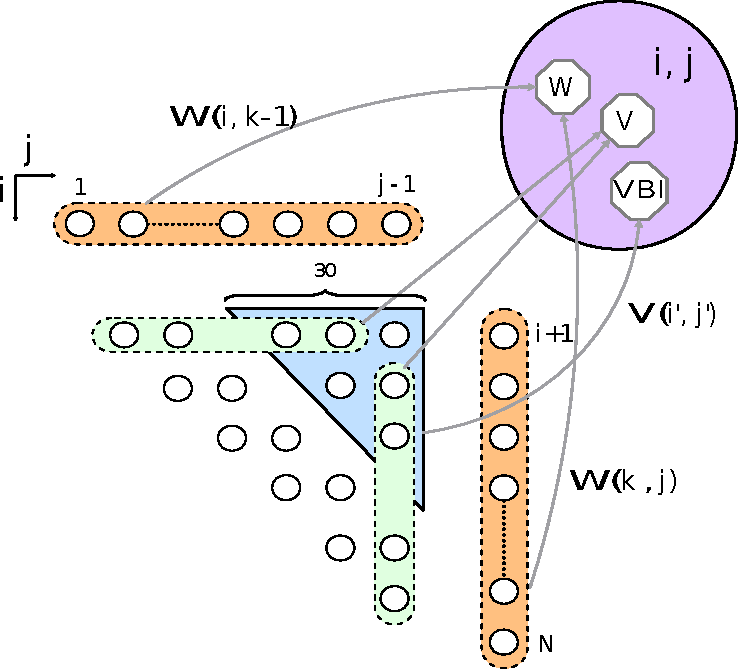
\includegraphics[width=7cm]{problems_zucker.pdf}\end{center}
	% source: <<Parallization of dynamic programming recurrences in computational biology>> paper
\item Optimizations: {\color{red} XXX}
\ole

% ------------------------------------------------------------------------------------------------
\newpage
\section{Plan}
\ol
\item {\color{gray}
\textbf{Problems:} finish the problem description. \\ We might look towards parallel tree-raking, but it does not share much with the above algorithms (sparse version of above computations, might not scale that well). Most of the common patterns are already enclosed by the above problems. Real input size is around 300'000 (we may want to target the million, using disk). We might want to also look at an $O(n^3)$-space complexity problem (like matching 3 strings $S,T,U$).
}

\item \textbf{User facing language:} goals are flexibility and compactness.\ul
	\item Design the user-facing language that we want to support, which should be similar to related papers <<Algebraic Dynamic Programming>> and <<ADP fusion>>. We want to reuse their transformation to map (problem description) $\mapsto$ (kernel implementation) for a single element.
	\item We also may want to try to make implicit transformation for code like \\
		{\tt @DP def Fib(n:Int) = if (n<=2) return 1 else Fib(n-1)+Fib(n-2)}.
	\item Windowing: the user should be able to force a windowing (i.e. force a non-serial problem to be a $k$-polyadic serial problem).	
	\item Consider 3 different cases: we care about backtrack, the costs or both.
	\item Backtracking: we might want to create an operator/class that given an item produces the previous in the backtrack, or the whole sequence in correct order, or only indices.
	\ule

$\implies$ \emph{end of October}.

\item \textbf{Prototyping:} get a prototype to understand difficulties and share common base. \\ Implement a working prototype of \nameref{aswat} on CPU (for correctness), and specific platform (CUDA/FPGA). This will give us an idea of how to implement the general case. We also need to benchmark and compare both implementations to see how we compare to existing implementations and see the direction to take (which decide is faster and by how much). Here we aim to do as good an implementaion for the specific platform (CPU/GPA) as possible.\\
$\implies$ \emph{end of October}.

\item \textbf{Baseline:} Also use benchmarks provided by existing implementations as baselines.\\
$\implies$ \emph{end of October}.

\item \textbf{Formalize IR:} According to experiences, describe the intermediate representation, also formalize the framework that will be provided to the code generators (i.e. memory management, ...).
\item \textbf{Full compiler stack:} enrich the compiler stack from both top-down (translate best user-facing language parsers) and bottom-up (parametric code generators), core of the work.
\item \textbf{Test and benchmark:} make sure our implementations are correct and compare them with previous papers implementations.
\ole

\newpage
\subsection{LMS compiler stack}
\textbf{User-language}: define additional parameters for the recurrence\ul
\item Windowing (to convert non-serial into serial problems)
\item Input sizes, and alphabets (backtrack, input, cost)
\item Backtrack (implicitly by backtrack alphabet size) and cost matrices bit-sizes (cost maximum may be inferred using <<Yield size/grammar analysis>>)
\item Recurrence functions, devices available
\item What to keep in memory (cost, backtrack or both).
\ule
$\Downarrow$ Conversion (using an existing technique)

\textbf{Intermediate representation}

$\Downarrow$ Optimizations\ul
\item Transform non-serial into serial \ul
	\item Use aggregation functions/transformations
	\item Use windowing from user (if no other technique succeed)
	\ule
\item Define the wavefront depth
\item Avoiding the cost matrix by moving it into the wavefront
\ule

\textbf{Code specification}\ul
\item Kernel function (1-element function), inputs, outputs, wave front, dependencies, bit sizes
\item Device-level interface => setup the block sizes(w/h), input and memory sizes
\item Define the device-specific implementation of the block (CPU/FPGA/CUDA)
\item Define the co-processor memory aggregation function
\item Define the scheduling of the blocks and aggregation (software pipelining)
\item Define the data movement back and forth to disk
\ule

$\Downarrow$ Generation\ul
\item Generate the kernel for specific device
\item Generate the scheduling and barriers
\ule

\textbf{Binary program}

%\ol
%\item Make sure we encompass all the most common patterns of DP: check if we have higher dimensions or more complex formula.
%\item Let the user tune the window size if he wants to reduce non-serial to serial.
%\item Concerns separation: common architecture enables flexibility (exchange components) \ul
%	\item Block processor: CPU, GPU, FPGA, must allow variation of width and height
%	\item Memory stats computation (min, sum, ... column/line combinations): CPU, GPU
%	\item Scheduler (CPU): interleave block computation and memory statistics
%	\ule
%\item Common description \ul
%	\item Block kernel processor
%	\item Full block
%	\ule
%\item Discussion: wavefront, design similarities, polyhedral theory
%\ole

%%\newcolumntype{C}[1]{>{\centering\let\newline\\\arraybackslash}m{#1}}
%\newcolumntype{C}{@{\hspace{7pt}}c@{\hspace{7pt}}}
%\def\mnl{\rule{0pt}{2.6ex}\rule[-1.2ex]{0pt}{0pt} \\ \hline}
%$\begin{array}{|C|C|C|C|C|C|} \hline
%0 & 0 & 0 & 0 & 0 & 0 \mnl
%0 &  &  &  &  & \mnl
%0 & M_{23}  &  &  &  & \mnl
%0 &  & \sum  &  &  & \mnl
%0 &  &  &  &  & \mnl
%0 &  &  &  &  & \mnl
%\end{array}$
\end{document}

\newpage
\section{Architecture design and technical decisions}
% ------------------------------------------------------------------------------------------------
\subsection{User facing language requirements}
The field of dynamic programming has been influenced in the recent years by a methodology known as Algebraic Dynamic Programming which uses a grammar and an algebra to separate between the parsing and the score computation:
\quote{The Algebraic Dynamic Programming approach (ADP) introduces a conceptual splitting of a DP algorithm into a recognition and an evaluation phase. The evaluation phase is specified by an evaluation algebra, the recognition phase by a yield grammar. Each grammar can be combined with a variety of algebras to solve different but related problems, for which heretofore DP recurrences had to be developed independently. Grammar and algebra together describe a DP algorithm on a high level of abstraction, supporting the development of ideas and the comparison of algorithms.}

Given such formalization \cite{adp} of dynamic programming on sequences, it seems natural to borrow from it and extend it to other types of DP problems. In short, this framework allow the user to define a grammar using parsers, which are then run over an input string and produce intermediate results that are memoized into a table, when multiple solutions are possible, the user can define an aggregation function ($h$) to retain only some candidates for further combination.

The benefits of ADP framework is that it does not constraint the result of the evaluation to be a single value, but can extend parsers to backtracking parsers or pretty-printers. Additionally, we want to support the following features:\ol
%\item {\color{red}\textbf{Cyclic problems:} are inherently very similar to string problems, except that the input is cyclic. To support such problem efficiently, we only need to mark the grammar cyclic such that it would apply on any unfolding of the cyclic input string.}
\item \textbf{Input pair algebra:} the original ADP framework only support single input, we want to support a pair of inputs such that we can treat problem such as Smith Waterman or Needleman-Wunsch. However, it does not make sense to treat more than two sequences because of the $\Omega(n^3)$ storage requirements that limits the problems size more dramatically.
\item \textbf{Windowing}: this can be easily encoded by passing the windowing parameter that limits the computation, then it could be possible to collect either the best or $k$-best results.
\item \textbf{Input restrictions:} since CUDA (and FPGA) cannot operate on an arbitrary Scala classes, we need to restrict the language to primary types (int, float, ... and structures of them). However, we want to preserve the expressiveness available for Scala and impose restrictions on the input and answers available to CUDA. A typical restriction we want to make is that processed structures are of fixed size so that we avoid memory management issues and thread divergence.
\item \textbf{Single-result on devices:} The general ADP framework supports multiple solutions for intermediate results. Such functionality is easy to support in Scala; however, memory management hampers the performance of the GPU implementation. To overcome this issue, the user could manually manage the memory, but this would defeat most of the benefits of automatic code generation. Hence the trade-off solution we propose is to restrict ADP to only one optimal result on CUDA, while leaving the freedom to obtain co-optimal (or even all possible solutions) with the Scala version.

\item \textbf{Automatic backtracking:} Since efficient code has to be devised we imposed restrictions on the output that could be generated by the parsers on devices. However, on the other side, the backtracking information would be of primary interest for the DSL user, hence we would like to to automate the backtracking to fulfill goals of usefulness, efficiency and ease-of-use in device-specific implementation:\ul
	\item Leaving the backtrack implementation to the user would force him to memoize the backtracking information together with the results (backtrack would  grow towards final result and duplicate unnecessarily information), hence requiring both $O(n^3)$ space and memory management features on devices. 
	\item Enforcing automatic backtracking presents the advantage to ensure constant size for intermediate results, hence ensuring an $O(n^2)$ storage requirement. Collecting the backtracking list can be easily done in $O(n)$ and then inverted whether we prefer bottom-up or top-down construction (the backtrack is usually a lattice of nodes that constitute a tree whose leaves are input elements).
	\ule
\item \textbf{Yield analysis:} in the vanilla ADP, the user has to define for each concatenation the minimal and maximal length of the subsequence on each side. Although non-emptiness information is necessary to avoid infinite recursion in the parsers, forcing an explicit definition can become cumbersome for the DSL user. We want to provide an automatic computation of concatenation boundaries, while at the same time leaving the possibility to manually specify it for maximum flexibility.
\ole

The support of these features has the following implications:\ul
\item \textbf{Dependency analysis:} Since we target GPUs (and FPGAs) which are massively parallel architecture, a top-down execution using hash tables is impractical (fallback computation if element is not present is hard to parallelize), hence we need to construct the result tree bottom-up, therefore ensure that the (partial) evaluation order between rules is respected.
\item \textbf{Normalization:} in order to automate the backtracking, we need the rule to present a certain shape so that we can define uniquely the backtracking information (in particular we want to distinguish between alternatives). Also we need to maintain coherency between the Scala and the CUDA version so that they can inter-operate: we would like to reuse the backtracking information (from CUDA) to do actual processing in Scala (for instance pretty-printing or effectively multiplying matrices).

\item \textbf{Optimizations:} An possible optimization is to break down complex rules into simpler ones if they are expressible so; hereby reducing the complexity of the overall algorithm, would the user production grammar not be optimal. Unfortunately this analysis is very involved: we need to solve the following problem:

Given $f$ , find a pair of functions $(f_1,f_2)$ or $(f_3,f_4)$ such that\footnote{The first equation denotes breaking in two functions, the second is Bellman's optimality principle.}
\[\begin{array}{rcll}
f(i,k_1,k_2,j) &=& f_1(i,f_2(i,k_1,k_2),k_2,j) & \land \\
	\min\limits_{i<k_1<k_2<j}\big[ f(i,k_1,k_2,j) \big] &=& \min\limits_{i<k_2<j} \big[ f_1(i,\min\limits_{i<k_1<k_2} \big[ (f_2(i,k_1,k_2  ) \big],k_2,j) \big] & \lor \vspace{12pt} \\
f(i,k_1,k_2,j) &=& f_3(i,k_1,f_4(k_1,k_2,j),j) & \land \\
	\min\limits_{i<k_1<k_2<j}\big[ f(i,k_1,k_2,j) \big] &=& \min\limits_{i<k_2<j} \big[ f_3(i,k_1,\min\limits_{k_1<k_2<j} \big[ (f_4(k_1,k_2,j) \big],j) \big]
\end{array}\]
% We can solve this more easily if functions are linear
Since this require complex mathematical analysis that are out of the scope of the project, we leave this optimization to the responsibility of the user.

Another optimization that is easier to implement is dead rule elimination. Traditional dead code elimination only reduces the size of the generated code. In the GPU implementation, this optimization will not only reduce the binary size but also the CUDA memory consumption as well as speed-up computation (since all rules are executed together).
\ule
% {\color{red} Size analysis to know what storage size we require: ex: Zucker requires $O(n^2)+O(n)$ storage...}

% ------------------------------------------------------------------------------------------------
\newpage
\subsection{Parsing grammar (ADP)}
In this section, we provide a concise description of the Algebraic Dynamic Programming. Would the reader be interested in the mathematical details of the notation, we encourage him to read the section 3 of \cite{adp}.

ADP is a formalization of parsers that introduces a distinction between the \textbf{parsing grammar} (recognition phase) and an associated \textbf{algebra} (evaluation phase). Such separation makes possible to define multiple algebra for the same grammar. This has two main applications:\ol
\item Experiment variants with the same grammar:  for example, Needleman-Wunsch and Smith-Watermann share the same grammar but have a different evaluation algebra
\item Use an evaluation and execution algebra: a dynamic programming problem is solved in two steps: computing one optimal solution and applying it over actual data. For example in matrix chain multiplication, the first step solves the underlying dynamic problem by evaluating the number of necessary multiplications, the second step \textit{effectively} multiplies matrices according to the order previously defined.
\ole

Practically, an ADP program is constituted of 3 components: a \textbf{signature} containing functions signatures, which are implemented by \textbf{algebrae} and a \textbf{grammar} containing parsers that make use of the functions defined in the signature. The concrete program instance mixes-in the algebra with the grammar. The grammar parsers intermediate results are memoized in an array (tabulation parser). A parser usually consist of a tree of:\ul
\item \textbf{Terminal:} operates on a subsequence of input elements and returns either its content or position (or a failure if the sequence does not fit the terminal).
\item \textbf{Filter:} accepts only subsequences matching a certain predicate. The condition is evaluated ahead of its actual content evaluation.
\item \textbf{Or:} expresses alternative between two different parsers and returns their result union.
\item \textbf{Concatenation:} constructs a larger sequence from two subsequences. The subsequences can be of fixed or varying size and concatenation operators might impose restrictions on the subsequences length to be considered.
\item \textbf{Map:} this parser transform its input using a user-defined function. It is typically used to transform a subword into a score that can later be aggregated.
\item \textbf{Aggregation:} the aggregation applies a functions that reduces the list of results, typically minimum or maximum, but the function can be arbitrarily defined.
\item \textbf{Tabulation:} the tabulation's primary function is to store intermediate results and possibly serve as connection point between different parsers.
\ule

Additionally, the signature must define input alphabet ({\tt Alphabet}), and output alphabet ({\tt Answer}) can be defined either in the signature or in the algebra. Finally, the grammar needs to have a starting point, denoted as axiom. Finally, the default aggregation function $h$ must be defined\footnote{Although aggregation usage is not mandatory in the framework, we force the existence of an aggregation function over the ouput type so that we can use it to aggregate windowed results.}. To make it more clear, we propose an example of the matrix chain multiplication problem\footnote{The original ADP framework was embedded in Haskell, however, we assume that the reader is more familiar with Scala notation and immediately present the syntax of our implementation.}. 

\newpage
\begin{lstlisting}[language=Scala, caption=Matrix chain mulitiplication DSL implementation]
trait MatrixSig extends Signature {
  type Alphabet = (Int,Int) // Matrix(rows, columns)
  val single:Alphabet=>Answer
  val mult:(Answer,Answer)=>Answer
}

trait MatrixAlgebra extends MatrixSig {
  type Answer = (Int,(Int,Int)) // Answer(cost, Matrix(rows, columns))
  override val h = minBy((a:Answer) => a._1)
  val single = (a: Alphabet) => (0, a)
  val mult = (a:Answer,b:Answer) =>
    { val ((m1,(r1,c1)),(m2,(r2,c2)))=(a,b); (m1+m2+r1*c1*c2, (r1,c2)) }
}

trait MatrixGrammar extends ADPParsers with MatrixSig {
  val axiom:Tabulate = tabulate("M",
    (el ^^ single | axiom ~ axiom ^^ mult) aggregate h)
}

object MatrixMult extends MatrixGrammar with MatrixAlgebra with App {
  println(parse(Array((10,100),(100,5),(5,50)))) // List((7500,(10,50)))
}
\end{lstlisting}
\begin{center}
\vspace{-24pt}
with or: $|\,\,$ map: $\land\land\,\,$ concatenation: $\sim$
\end{center}

\vspace{3cm}
This program grammar can also be expressed in BNF:
\[\begin{array}{lrl}
axiom &::=& \text{matrix} \\
 &|& axiom \,\,\, axiom
\end{array}\]

and it encodes the following recurrence (cost only):
	\[M_{(i,j)}=\left\{\begin{array}{ll}
		0 & \text{if } i+1= j\\
		\min_{i<k<j} M_{(i,k)}+M_{(k,j)}+r_i \cdot c_k \cdot c_j & \text{otherwise}
	\end{array}\right. \]

Notice that the semantics of indices differ slightly from the problem presented in \ref{mat_mult_plain}; this is because empty chain are made expressible (denoted $M_{(i,i)}$, single matrices are denoted $M_{(i,i+1)}$).

% ------------------------------------------------------------------------------------------------
\newpage
\subsection{Recurrences analysis}
\subsubsection{Dead rules elimination}
Dead rules\footnote{\textit{Rule} denotes a tabulation belonging to the grammar; both terms refer to the same concept, with the subtle difference that \textit{rule} emphasizes its grammar membership.} elimination analysis is straightforward: starting from the grammar's axiom, recursively collect all tabulations involved in the computation in $R$ (set of rules that are mandatory in the grammar). The dead rules $D=S \setminus R$ (where $S$ is the set of all tabulations) can safely be removed from the grammar rules. Although seemingly useless for the Scala implementation, this step is necessary to maintain coherency between Scala and CUDA rules numbering (that happen in a later stage on the valid rules). In CUDA, this analysis not only provides dead code elimination, but it also prevents useless computation execution, since all rules are computed sequentially for a particular subsequence before the next subsequence is processed.

\subsubsection{Yield analysis}
Since the original ADP introduces many concatenation combinators\footnote{ADP's original combinators are: $\sim\sim, \sim\sim*, *\sim\sim, *\sim*, -\sim\sim, \sim\sim-, +\sim\sim, \sim\sim+, +\sim+$.} to differentiate empty/non-empty, and floating/fixed-length concatenations, it is quite involved for the programmer to make sure that the concatenation operators exactly match the size of each pair of subsequence involved. Additionally the priority of operators varies in Scala, depending the operator's first character whereas it is possible to specify arbitrary priorities in Haskell. To overcome these issues, we propose to automate the computation of the minimum/maximum length of (subsequences) parsers.

Parsers are made of terminals, concat, operations (aggregate, map, filter) and tabulations; minimum/maximum yield of terminals is set, hence it only remains to assign appropriate yield sizes to tabulations; other operations simply propagate that information. It is possible to obtain the yield size of tabulations using the following algorithm (assuming recursive parsers contain at least one tabulation that is part of the loop):\ol
\item Set the yield minimum size of all tabulations to a large number $M_0$ (such that all tabulation would reasonably have a minimum yield size smaller than $M_0$)
\item Repeat $k$ times ($k$ is the number of rules of the grammar): for each rule, compute its minimum yield size and update its value (without recursion at tabulations). This would lead to a correct minimum yield size because the terminals provide a minimum size and this might need at most $k$ iteration to propagate across all rules.
\item Set the maximal yield of all the rules to the minimal value. For each rule, compute recursively up to depth $k$ (where the depth is computed as the number of tabulation traversed) the maximum yield size. If the depth reaches the maximum $k$, there is a loop between tabulations, hence return infinity.
\ole

The last part of this algorithm seems to have an exponential complexity, however, if we consider depth-first search and return as soon as we reach infinity, we might reduce its complexity to $O(k^2)$. Obtaining the yield size of tabulations provides the following benefits:\ul
\item Minimum size: prevents self-loops (computing one matrix cell using its own result) and avoid considering subsequences that would yield empty result (hence slightly reducing time complexity).
\item Maximum size: allows to reduce the size of the result and backtrack matrix to $O(m\cdot n)$ instead of $O(n^2)$ (where $m$ is the maximum yield size), possibly providing substantial space savings. As the rules with bounded maximum yield are very rare, we did not implement this optimization, although we might consider it for future work.
\ule

\subsection{Dependency analysis}
Let us introduce the concept of dependency: a dependency between tabulations $A,B$ denoted $A\to B$ exists if $B_{(i,j)} = f(A_{(i,j)})$, that is if the result of $B$ depends of the result on the \textit{same} subproblem computed in $A$. A grammar is unsolvable if there exist a dependency loop between parsers ($A\to ... \to A$). Such case only happen when there is no concatenation or a concatenation with an empty word. Being able to track the dependencies of tabulations and infer a computation order between them has two benefits:\ul
\item Although seemingly unnecessary in a top-down approach (Scala), this analysis detects dependency loops which would result in infinite call loops (stack overflow) at execution.
\item Ordering tabulations is critical in a bottom-up approach (CUDA) to make sure that all dependencies are valid before an element computation is triggered.
\ule

% ------------------------------------------------------------------------------------------------
\subsection{Backtracking}
In order to produce an efficient transformation from ADP-like problem description to plain C recurrences, we need to construct bottom-up recurrences from top-down parser rules. To do that, we slightly need to modify the ADP parsers in order to separate the backtracking and the scoring, because we want to obtain an efficient algorithm: backtrack writes are in $O(n^2)$ whereas score reads are proportional to the algorithmic complexity ($O(n^3)$ or more for non-serial). To deal with this problem, we are facing two options:\ul
\item \textbf{Explicit backtracking:} requires clear syntactical separation between the score and the backtrack which is not implemented in ADP, unless we consider the whole backtrack being part of the scoring (which has a big performance impact and non-constant memory requirement issues that make such GPU implementation hard and not desirable). Additionally, since the backtracking data is user-defined, there is no way to generate the backtracking algorithm automatically, hence the user also needs to provide it.
\item \textbf{Implicit backtracking:} implies that every rule needs to be normalized, and transformed such that given a rule identifier and a set of indices (subproblems breaking), it is possible to retrieve the sub-solutions combination that contribute to the problem solution. To do that we need to apply the following transformations\ol
	\item Normalize rules and identify them uniquely by exploding alternatives: each rule is decomposed into the union of multiple sub-rules uniquely identified by an index, where sub-rules do not contain alternatives (Or parsers). Let $s$ a subrule and $r_s$ its identifier, we also establish a mapping $T$ from identifier to subrule: $(r_s \to s) \in T$.
	\item Let ${\rm cc}(r_s)$ the number of concatenation contained in the sub-rule $r_s$. The data element corresponding to a rule is a pair (score, backtrack) and is named after the tabulation.\ul
		\item The score part consists of a user-defined type (a composite of primitive types, case classes and tuples)
		\item The backtrack part is a tuple $(r_s,(k_1, k_2, \ldots , k_m))$ where $m$ is the maximal number of concatenations occurring in the enclosing rule of $r_s$; more formally $m=\max_z\big[{\rm cc}(r_z) | r_z \in {\rm rule}(r_s)\big]$, and let $m_s = {\rm cc}(r_s) \le m$.
	\ule
	\item During the matrix computation of cell $(i,j)$, if the sub-rule $r_s$ applies, the backtrack will be set as $(r_s,(k_1,k_2,\ldots,k_{m_s}))$; with $i\le k_1\le k_2\le \ldots k_{m_s}\le j$. Note that if the backtrack occupies a fixed-length memory, the backtrack will contain exactly $m$ indices, hence $k_i\,|\,m_s<i\le m$ will be unspecified.
	\item During backtracking, when reading the cell $(i,j)$ with backtrack $(r_s,(k_1,k_2,\ldots,k_m))$, given $r_s$, we recover $s=T(r_s)$, the sub-rule that applies. Hence we can determine $m_s$, which allows us to enqueue the subsequences $(i,k_1), (k_1,k_2), ..., (k_{m_s},j)$ for recursive backtracking. If $s$ refers to a terminal, we stop the backtracking.
	\item The backtracking can be returned to the user as a mapping table $T$ and a list of triplets $((i,j),r_s,(k_1,k_2,\ldots,k_{m_s}))$ where $(i,j)$ denotes the subsequence on which the sub-rule $T(r_s)$ has to be applied with concatenation indices $(k_1,k_2,\ldots,k_{m_s})$.
\ole
In short, we break parsers into normalized rules, the backtracking information is the subword, the sub-rule id (which rule to unfold) and a list of indices (how to unfold it).
\ule
In order to reduce the storage required by the backtracking indices, we can avoid storing fixed indices (where at least one of the two subsequences involved in a concatenation has a fixed size) and leverage the knowledge contained in $s$ to reconstruct the appropriate backtrack.

Assuming that the backtracking information is meant to guide further processing, we provide this information into a list constructed bottom-up: it can be simply processed in-order, applying for each rule the underlying transformation, and storing intermediate results (i.e. in a hash map) until they are processed by another rule. Since there is only one consumer for each intermediate result, every read in the hash map can remove the corresponding value, hence reducing the memory consumption. Ultimately, only the problem solution will be stored in the hash map.

% ----------------------------------------------
\subsubsection{Backtracking with multiple backtrack elements}
{\center\color{red} XXXXXXXXXXXXXXXXXXXXXXXXXXXXXXXXXXXXXXXXXXXXXXXXXXXXXXXXX\\ CONTINUE HERE\\ XXXXXXXXXXXXXXXXXXXXXXXXXXXXXXXXXXXXXXXXXXXXXXXXXXXXXXXXX}

The backtracking technique described above work fine when there is a single element stored per matrix cell (which is usually the case with min/max problems). However, in the generalization introduced by ADP, it is possible that a matrix cell stores multiple results. In such case, we need to select a correct result to avoid backtracking inconsistencies.

Additionally, we need to keep track of the multiplicities of the solutions, that is if we want to obtain the $k$ best solutions, we need to make sure that we return $k$ different backtracks. To do that, we maintain a multiplicity counter in each backtrack process: \ul
\item While there is a single solution for all possible incoming paths, we continue in this direction with the same multiplicity (we have no choice).
\item When there is $r$ different solutions available, and the path multiplicity at this point is $k$ we have the following cases: \ol
	\item If $k\ge r$: we explore all paths with multiplicity $k-r+1$. This is because each branch may produce only one solution and we don't know ahead of time which path will provide multiple solutions. Finally, we retain only the $k$ best solutions.
	\item If $k<r$ (there is more paths than needed): we can only explore the $k$ first paths with multiplicity 1 and safely ignore the other (as we only need $k$ results).
	\ole
\ule

Now it remains the problem to generate all possible results and check whether they are correct correct. To do that we can simply re-apply the parsers while maintaining the source elements of all production and then retain only those with desired score and backtrack. Since we know the backtrack for one element, we can do the following optimization at backtrack parser computation:\ol
\item Defuse or's: since we know exactly (by the subrule id, maintained in the backtrack) which alternative has been taken to obtain the result, we can skip undesired branches of or parsers.
\item Feed concatenation indices: since the backtrack stores the concatenation indices, we can reuse in the concatenation parsers. This removes the $f(n)$ factor in the backtrack complexity (as concatenation backtrack parsers <<know>> where to split).
\item Skip filters: since filter are applied before their inner solution is computed, their are only position-dependent. Hence if a backtrack involves a filter, since its position is fixed, the filter must have been passed at matrix construction time.
\ole

% ----------------------------------------------
\subsubsection{Backtracking complexity}
We want to have an estimation of the complexity of the two operations to see what is the overhead of multiple backtracking. For single-element backtrack, we only need to revert the parser to find involved subwords, which is linear in the parser size (because the backtracking identifies uniquely the alternative in or's and indices in concatenations). At every backtrack step, either:\ul
\item The word is removed at least one character, which leads to maximal backtrack length of $n$.
\item The word is split in $s$ subwords, with recurrence $f(n)=2f(n/2)+1$ by solving this recurrence we see that there can be at most $n$ final nodes and $n$ intermediate nodes (when $s=2$). Hence the backtrack length is at most $2n$.
\ule

Let one parser reversal complexity be $O(p)$, single backtrack has $O(2n\cdot p)$ complexity. For the $k$-elements backtrack, since we regenerate all possible solutions, that is $O(k^{c+1})$ candidates (with $c$ the maximal number of concatenation in the parser), the overall complexity is $O(2n \cdot k^{c+1} \cdot p)$. Hence there is a $k^{c+1}$ factor to pay if we want to backtrack the $k$ best solutions\footnote{Note that the same $k^{c+1}$ factor lies in the forward matrix computation complexity.}.

% ----------------------------------------------
\subsubsection{Backtrack utilization}
Since the dynamic programming input may be a subset of the larger problem that we want to resolve\footnote{For instance in matrix chain multiplication, we only care about matrix dimensions for dynamic programming, however, we ultimately want to multiply the real matrices and obtain a result.}, we need to be able to apply the result of the dynamic programming computation on values in a different domain. The easiest way to do that, is to reuse the same grammar on a different domain, and only compute the resulting trace obtained from the DP solver.

This step is pretty straightforward: since ADP parsers emphasize on the split between signature and grammar and decouples them, we only need to modify the signature to operate on another domain, and reuse the same grammar. The key point here is to notice that a backtrack trace on one parser can be reused on another, providing that they have the same grammar. For instance, to compute optimally a matrix chain multiplication, we solve the DP problem in a domain where matrices are represented by their dimensions, we obtain an optimal trace and feed it to a parser operating on the <<real matrices>> domain that will do the actual computation.

% ------------------------------------------------------------------------------------------------
\subsection{CUDA storage: from list to single-value}
Since lists are one of the primary type of the Scala language, it is natural to gather parsers results into lists in Scala implementation. However, when it comes to efficient CUDA implementation, lists must be avoided because memory allocation (and management) is not very efficient. A workaround might be to use fixed-length lists but we assume here that the programmer is most often interested in a single optimal solution (this also alleviates the complexity of constructing multiple distinct backtrack traces). Even if this design choice apparently greatly simplifies the design issues might arise for how to represent and deal with empty lists and how to minimize the amount of used memory:\ul

\item \textbf{Minimizing memory consumption:} Under the restriction that we only store the best result, we first need to transform aggregation such that they return at most one element. Useful aggregator belonging to this class are quite limited: minimum/maximum (optionally with respect to an object's property), count and sum\footnote{Notice that all these operations can be implemented with a folding operation on a single variable.}, hence it is possible to provide them to the user. To benefit of this fixed memory aggregation, we need to do some structural transformation of inner parsers. In general, a tabulation $T$ is the root of its evaluation tree, with leaves being either other tabulations or terminals, note that any of the 5 intermediate element can appear multiple times (or not being present) and in any order.
\[T < \textbf{Aggregate} < \textbf{Or} < \textbf{Filter} < \textbf{Map} < \textbf{Concat} < \text{(Tabulate | Terminal)}\]

For obvious performance reasons, we want to maintain aggregations wherever they are present. However, we can partially normalize the rest of the evaluation tree:\ul
	\item We must ensure that all parsers potentially generating multiple possibilities are aggregated. To do that, we simply wrap the original parser in an $h$-aggregation (where $h$ is the default aggregation function that must be specified by the user)
	\item Since the aggregation now operates on a single element, we want to push it as close to the leaves as possible, as long as we do not change operational domain\footnote{We cannot push an aggregation through a mapping or a concatenation operation}.
	\item Filters can be hoisted within the same concatenation / alternative
	\item Alternatives must be hoisted outside of maps and concatenations, the reason being that we need to avoid maintaining list of candidates (that will be later aggregated).
	\ule

\begin{center}
\begin{tabular}{l|lllll}
Outer $\diagdown$ inner	& Aggregate	& Or			& Map	& Filter		& Concat \\ \hline
Aggregate			& merge?		& swap$_R$	& ---		& swap$_P$	& ---\\
Or					& ---			& simplify?	& ---		& swap$_P$?	& ---\\
Map					& ---			& swap$_R$	& fuse	& swap$_P$	& ---\\
Filter					& ---			& ---			& ---		& merge?		& ---\\
Concat				& ---			& swap$_R$	& ---		& ---			& ---\\
\end{tabular} \\[10pt]
\footnotesize{$R=\ $required, $P=\ $performance optimization}
\end{center}

Note that there can be no swap with Map and Concat internal parsers due to domain change. Fusing is done by the C compiler (declaring mapping functions inline).

\item \textbf{Handling nested aggregations:} since the parser might contain nested aggregation, they must be preserved in order not to increase its time complexity. To do that, each internal aggregation has to define its own intermediate variables and backtrack, whereas outermost aggregation can directly write in the cell of the cost/backtrack matrix.
\item \textbf{Failure handling:} a parser can either be successful and return a valid result or fail and return no result; failure can happen in terminals, (source) tabulations and filters. These 3 cases can be reduced to one by wrapping terminals and tabulations into a filter that checks validity conditions. It remains to discuss failure encoding strategies:\ul
	\item \textbf{Special <<empty>> value: }The benefit of such encoding is a reduced number of memory accesses, indeed since we need to access anyway the value to make computations, we do not generate additional memory accesses to check the validity of the value. The drawback of such approach is that it becomes necessary to specify a special <<empty>> value that cannot be used, except to denote the absence of result. Since types can be arbitrary at every step of the parser, it becomes cumbersome to ask the DSL user to provide a special value for every intermediate result.
	\item \textbf{Backtrack encoding:} Reusing the backtrack to encode the validity of a result is a more general approach, and allow greater flexibility for the user. Indeed, since we maintain subrules in the backtrack, it suffice to use a special subrule number to denote that related value is invalid.
	This approach also work with nested aggregations by storing an <<intermediate subrule>> temporary that would only grant validity of the related value.
	\ule
Since backtrack encoding comes at the price of an additional memory access to test the validity (memory accesses usually accounts for most of the time on CUDA devices), it is also relevant to allow the user to completely disable this test to speed-up computations.
\ule

% ------------------------------------------------------------------------------------------------
\subsection{Memory constraints}
We denote by \textit{device} the computational device on which the processing of the DP matrix (or of a computational block) is done and $M_D$ its memory. This can be the GPU or the FPGA internal memory. Usually the main memory is larger than device memory and can ultimately be extended by either disk or network storage.

We propose to evaluate the device memory requirements to solve the above problem classes. We need first to define additional problem properties related to implementation:\ul
\item \textbf{Number of matrices:} multiple matrices can be encoded as 1 matrix with multiple values per cell. Hence the implementation differentiates only between cost and backtrack matrices with respective element sizes $S_C$ and $S_B$.
\item \textbf{Delay of dependencies:} In case the problem does not fit into memory, partial matrix content needs to be transferred across sub-problems. Such data amount is usually proportional to the delay of dependencies. If this delay is small, it might be worth to duplicate matrix data in the wavefront, otherwise it might be more efficient to allow access to the previous computational blocks of the matrix.
\item \textbf{Wavefront size:} Finally some aggregation that is made along some dimension of the matrix does not need to be written at every cell but can be propagated and aggregated along with computation (ex: maximum along one row or column). Hence such information can be maintained in a single place (in the wavefront) and progress together with the computation. We denote by $S_W$ the size of wavefront elements.
\item \textbf{Input size:} the size of an input letter (from input alphabet) is denoted by $S_I$.
\ule

% ----------------------------------------------
\subsubsection{Small problems (in-memory)}
Problem that can fit in memory can be solved in a single pass on the device. Such problem must satisfy the equation:
	\[(S_I+S_W) \cdot (m+n) + (S_C+S_B) \cdot (m\cdot n) \le M_D\]

For instance, assuming that $m=n$, $M_D=1024{\rm Mb}$, that backtrack is 2b (<16384, 3 directions) and that the cost can be represented on 4 b (int or float), that input is 1b (char) and that there is no wavefront, we can treat problems of size $n$ such that $2n+5n^2 \le 2^{30} \implies  n\le 14650$. We might also possibly need to take into account extra padding memory used for coalesced accesses. But it is reasonable to estimate that problems up to 14K fit in memory.

% ----------------------------------------------
\subsubsection{Large problems}
To handle large problems, we need to split the matrix into blocks of size $B_H \times B_W$. For simplification, we assume a square matrix made of square blocks with $b$ blocks per row/column.

% ----------------------------------------------
\subsubsection{Non-serial problems}
Non-serial problems need to potentially access all elements that have been previously computed. We restrict\footnote{As we have not encountered a problem with non-serial dependencies along the diagonal.} ourselves to the following dependencies: \ul
\item Non-serial dependencies along row and column
\item Serial dependencies along diagonal, with delay smaller or equal to one block size
\ule
Such restriction implies that all the block of the line and the row, and one additional block to cover diagonal dependencies must be held in memory (independently of the matrix shape).

For simplification, let $m=n$ and assume that we have $b$ square blocks per row and per column. Hence we have the following memory restriction:
\[ 2\frac{n}{b}(S_I+S_W) + 2 \cdot \frac{n^2}{b}S_C + \frac{n^2}{b^2} S_B \le M_D\]

We also need to take into account the transfer between main memory (or disk) and device memory. Dependency blocks only need to be read, computed blocks need to be written back. Ignoring the backtrack and focusing only on the cost blocks, the transfers (in blocks) are:
\[\begin{array}{rclll}
		b^2 +% computed line writeback (once)
		(b-1)^2 + % diagonal block loads (1 per block)
		\sum\limits_{i=0}^{b-1} i \cdot b % column dependencies loads (for line i)
		&=&\tfrac{1}{2}b^3+\tfrac{3}{2}b^2-2b+1 &\qquad& \rm (Rectangle)
	\\
		\sum\limits_{i=1}^{b} \Big(1+2\cdot(i-1)\Big) \cdot (b+1-i) % on i_th diagonal
		&=& \tfrac{1}{3} b^3 + \tfrac{1}{2}b^2 + \tfrac{1}{6}b &\qquad& \rm (Triangle)
	\\
		\sum\limits_{i=1}^{b} \Big(1+2\cdot(i-1)\Big) \cdot b % on i_th diagonal
		&=& b^3 &\qquad& \rm (Parallelogram)
\end{array}\]

Putting these two formula together, and using most of the device memory available, we obtain the following results with $S_C=4, S_B\footnote{To deal with larger matrices, backtrack data need to be extended.}=4, S_I=1, S_W=0$ and $M_D=2^{30}$:
\begin{center}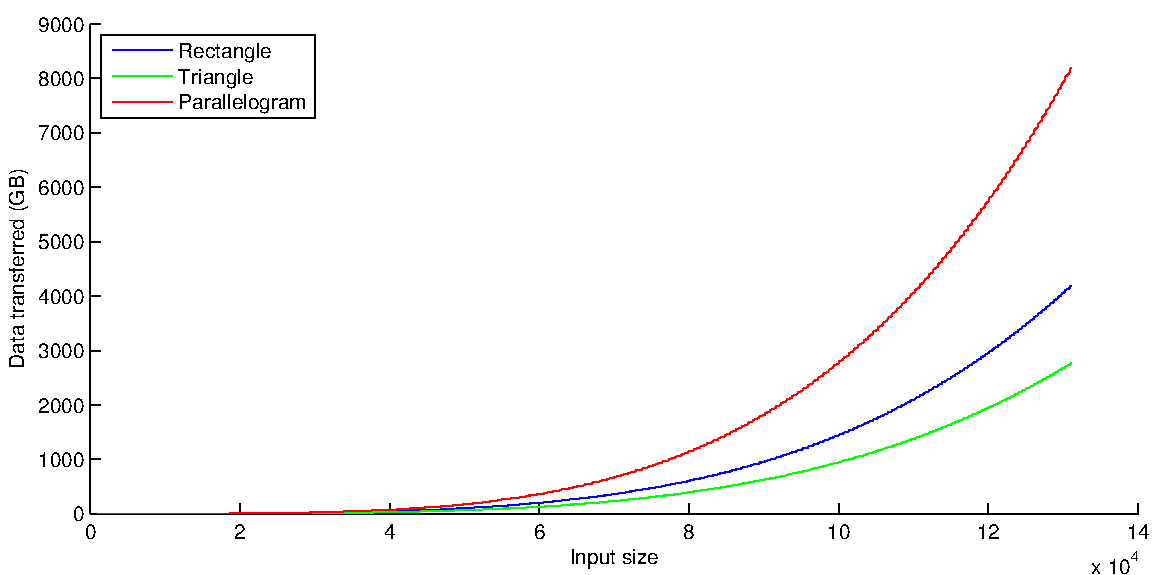
\includegraphics[width=14cm]{inc/ns_large.pdf}\end{center}

Given an experimental bandwidth of 5.3743 Gb/s between CPU and GPU, processing matrices one order of magnitude larger (128K) would result in respectively 13\up{(R)}, 8.5\up{(T)} and 25.4\up{(P)} minutes of transfer delay. Extrapolating the preliminary results of small problems, a computation on input of size 128K would require respectively 7 days 13h\up{(R)}, 2 days 22h\up{(T)} and 6 days 10h\up{(P)}, assuming there is no other scalability issues. Although this overhead seems appealing compared to the computation time, the total time blows up (because of the  $O(n^3)$ complexity) and make the processing of such large problem less relevant. Given that real problems -- like RNA folding -- operate at input sizes up to 4096, it would not be of much relevancy to implement a version for larger cases, although perfectly feasible.

% ----------------------------------------------
\subsubsection{Serial problems}
The serial problem have the interesting property to access to a fixed number of previous elements. These elements can be either stored either explicitly in a scoring matrix or implicitly as moving aggregation into a wavefront. Since the dependencies are fixed, the computation direction gains an additional degree of freedom: matrix can be solved in diagonal (as non-serial problems) or line-wise or column-wiser. This allows to store the whole necessary state to make progress into a limited number of lines (or columns), and sweep vertically (resp. horizontally) along the matrix.

Since serial problems are of complexity $O(n^2)$ (due to the matrix dimension and the finite number of dependencies), it is possible to tackle much larger problem than non-serial during the same running time. Hence, it seems obvious to let serial problems grow larger than the memory.

Mixing the dependency property and size requirements, we can split the matrix into sub-matrices, store special lines (and/or columns) into memory (or hard disk), and repeat computations to solve the backtrack (similarly as in \cite{swat_gpu},\cite{swat_mega}, but this implementation use problem-specific knowledge that might not generalize).

To store intermediate lines and columns, we are facing two different strategies to explore:\ul
\item \textbf{Fixed subproblem size:} we decompose the algorithm as follows\ol
\item Define a grid of <<major column and rows>>, where each cell's data (input, output, cost and backtrack matrices) fits into the device memory.
\item Compute the values of the grid's major columns and rows in one pass.
\item Second (on-demand) computation to process backtracking inside relevant cells.
\ole
Let $b$ the number of cells that we have on each row/column, the total computation running time would be $(b^2 + 2b) \cdot t_b$ where $t_b$ is the time to compute one cell's matrix. This division has the advantage of providing the minimal computation time at the expense of external storage proportional to $O(n)$ (if we store only lines or columns) or $O(n^2)$ (if we store both).

\item \textbf{Myers and Miller’s algorithm:} (divide and conquer)
This algorithm break the DP problem into 2 (or 4) subproblems such that once the middle line/column is computed, the problem can be solved for 1 submatrix and backtracking among up to 2 of the 3 other. This breaking is applied recursively until the submatrix data fits into memory. The storage requirements are $4 \cdot O(n)$ (we store along both dimension $1+\tfrac{1}{2}+\tfrac{1}{4}+...$ lines/columns).

The algorithm proceeds as follows: first it solves the problem to obtain the first backtracking element, then it breaks the matrix in 4 submatrices, and refine it until backtrack is tractable. Since there is at most $\log n/b$ refinements and since every part of the matrix may be involved in backtrack, running time is $O(n^2 \log_2 n)$.
\item \textbf{Hybrid approach:} a hybrid approach might be created to take advantage of additional available memory, however, the running time decreases logarithmically to the space used, this means that using twice more storage space would only result in a $2\times$ speedup (measuring only the computation time). Hence an hybrid approach would be to decide a $k$ such that at each step we partition the desired submatix into a intermediate grid of $k$ rows/columns. The space usage would be in $2 k \log_k (n/b)$ and the running time complexity would be $O(n^2 \cdot \log_k n)$. Then the user would be able to fix a storage space $S \ge 4 \log_2 (n/b)$ and obtain the corresponding $k$ for a given $n$.
\ule

{\color{red}
try to setup wavefront size (if needed) => just enlarge the matrix by 1 so that we go wavefront-to-wavefront

XXX: what's the maximal size of the wavefront ??

XXX: can we avoid to store some matrices and put them in the wavefront ??

Split into blocks:\ul
\item Decide the shape of the blocks
\item Decide the size of the blocks
\item Decide of a strategy to store intermediate lines/columns: space/time tradeoff.
\ule

XXX: make it work up to 14K for all 3 problems using multiple kernels
XXX: example of non-symmetric serial problem

The three last elements, combined with the above one, provide a precise estimation of the memory consumption, and the implementation difficulty 

all the problem are subject to the input dimensions $n$.

the two latter one gives an estimation of the constant factor.

The delay of dependencies might also have an impact: if the matrix is too large to fit in the memory (device or main memory), it becomes necessary to maintain partial matrix content (all the intermediate elements) within the wavefront. Also the number of cost matrices might affect the performance, simply because maintaining them requires computations and memory accesses.
}

% ------------------------------------------------------------------------------------------------
\subsection{Memory layout}
{\color{red} XXX}


% ------------------------------------------------------------------------------------------------
\newpage
{\color{red} 
\subsection{LMS compiler stack}
\textbf{User-language}: define additional parameters for the recurrence\ul
\item Windowing (to convert non-serial into serial problems)
\item Input sizes, and alphabets (backtrack, input, cost)
\item Backtrack (implicitly by backtrack alphabet size) and cost matrices bit-sizes (cost maximum may be inferred using <<Yield size/grammar analysis>>)
\item Recurrence functions, devices available
\item What to keep in memory (cost, backtrack or both).
\ule
$\Downarrow$ Conversion (using an existing technique)

\textbf{Intermediate representation}

$\Downarrow$ Optimizations\ul
\item Transform non-serial into serial \ul
	\item Use aggregation functions/transformations
	\item Use windowing from user (if no other technique succeed)
	\ule
\item Define the wavefront depth
\item Avoiding the cost matrix by moving it into the wavefront
\ule

\textbf{Code specification}\ul
\item Kernel function (1-element function), inputs, outputs, wave front, dependencies, bit sizes
\item Device-level interface => setup the block sizes(w/h), input and memory sizes
\item Define the device-specific implementation of the block (CPU/FPGA/CUDA)
\item Define the co-processor memory aggregation function
\item Define the scheduling of the blocks and aggregation (software pipelining)
\item Define the data movement back and forth to disk
\ule

$\Downarrow$ Generation\ul
\item Generate the kernel for specific device
\item Generate the scheduling and barriers
\ule

\textbf{Binary program}
}
%\ol
%\item Make sure we encompass all the most common patterns of DP: check if we have higher dimensions or more complex formula.
%\item Let the user tune the window size if he wants to reduce non-serial to serial.
%\item Concerns separation: common architecture enables flexibility (exchange components) \ul
%	\item Block processor: CPU, GPU, FPGA, must allow variation of width and height
%	\item Memory stats computation (min, sum, ... column/line combinations): CPU, GPU
%	\item Scheduler (CPU): interleave block computation and memory statistics
%	\ule
%\item Common description \ul
%	\item Block kernel processor
%	\item Full block
%	\ule
%\item Discussion: wavefront, design similarities, polyhedral theory
%\ole

%%\newcolumntype{C}[1]{>{\centering\let\newline\\\arraybackslash}m{#1}}
%\newcolumntype{C}{@{\hspace{7pt}}c@{\hspace{7pt}}}
%\def\mnl{\rule{0pt}{2.6ex}\rule[-1.2ex]{0pt}{0pt} \\ \hline}
%$\begin{array}{|C|C|C|C|C|C|} \hline
%0 & 0 & 0 & 0 & 0 & 0 \mnl
%0 &  &  &  &  & \mnl
%0 & M_{23}  &  &  &  & \mnl
%0 &  & \sum  &  &  & \mnl
%0 &  &  &  &  & \mnl
%0 &  &  &  &  & \mnl
%\end{array}$
%\end{document}

\newpage
\section{Implementation}
% ------------------------------------------------------------------------------------------------
\subsection{Ad-hoc CUDA}
In the project planning, an ad-hoc implementation phase immediately followed the problem analysis (we also present the parallelogram matrix case). The goal of this phase is threefold:\ol
\item Better understand the challenges in CUDA implementation of dynamic programming problems and get on par with state-of-art implementations.
\item Have a baseline implementation that is independent of the hardware and that could be benchmarked. We also tried to contact the authors of \cite{swat_mega} and \cite{gpu_atlp} to obtain their implementation. The former provided us with their implementation, which turned out to address large serial problems whereas our focus was on smaller non-serial problems, the latter did not respond to our solicitations.
\item Have an optimal implementation that can serve as target to be imitated and generalized by the code generation.
\ole

Leveraging the insights provided by \cite{gpu_atlp} and \cite{gpu_barrier}, we started with a basic implementation (where each CUDA thread processes one matrix line) with three additional optimizations:\ul
\item Memory accesses must be coalesced (memory accesses account for a significant part of the total running time, according to both manufacturer documentation and experiments \cite{perfeval})
\item Synchronization between threads can be done according to \cite{gpu_barrier}, additionally, we can slightly loosen the synchronization restrictions, as the paper describes a thread barrier whereas we only require a condition on previous thread progress (except for the parallelogram case, where we still require a barrier).
\item Computation progresses element-wise along the diagonal (maximizes the parallelism level)
\item Thread block size = warp size (32) to benefit from implicit synchronization within warps
\ule

% ----------------------------------------------
\subsubsection{Related work}
Since \cite{swat_mega} focuses on a different class of problem, we compare our implementation against \cite{gpu_atlp}, which provides an efficient matrix multiplication implementation. However, since we have neither the source code (or binary) nor the same evaluation hardware, we need to normalize the results. To do that, we present hardware differences and their result:

\def\unt#1{& \footnotesize #1}
\begin{table}[H]\begin{center}\begin{tabular}{lrrr} \toprule
\bf Graphic card &				& \bf Our 		& \bf  ATLP\cite{gpu_atlp} \\ \midrule
Model &						& GeForce GT 650M	& Tesla C1060 \\
Architecture, capability  &			& Kepler (3.0)	& GT200 (1.3) \\
Memory \unt{Mb}				& 1024		& 4096 \\
CUDA cores &					& 384		& 240 \\
Clock (core, memory) \unt{MHz}	& 756, 1953	& 1300, 1600 \\
Memory bus \unt{bit}				& 128		& 512 \\
Memory bandwidth \unt{GB/s}		& 28.8		& 102.4 \\
Processing power \unt{GFLOPS}	&564.5		& 622.08 \\ \midrule
\bf Processing speedup & 		& 1			& 1.07 \\
\bf Memory speedup & 			& 1			& 3.55 \\ \bottomrule
\end{tabular}\end{center}\caption{Graphic cards technical specifications (source: \href{http://en.wikipedia.org/wiki/Comparison_of_Nvidia_graphics_processing_units}{Wikipedia})}\end{table}

\begin{table}[H]\begin{center}\begin{tabular}{lrrrrrrrrrr} \toprule
\bf Matrix size & 128 & 256 & 512 & 1024 & 1536 & 2048 & 2560 & 3072 & 3584 & 4096 \\ \midrule
\bf No split & 0.07 & 0.09 & 0.19 & 0.59 & 1.27 & 2.25 & 3.51 & 5.07 & 6.92 & 9.06 \\
\bf Split at 1 & 0.06 & 0.07 & 0.08 & 0.14 & 0.26 & 0.47 & 0.77 & 1.21 & 1.80 & 2.57 \\ \bottomrule
\end{tabular}\end{center}\caption{ATLP\cite{gpu_atlp} results: matrix chain multiplication, execution time (in seconds)}\end{table}

% ----------------------------------------------
\subsubsection{Results}
We present here the timings of our implementation. For correctness, we first implemented a CPU version that we used to compare CUDA results against. Input data is made of random numbers. The implemented dynamic programming problems are:\ul
\item Rectangle: Smith-Waterman with arbitrary cost
\item Triangle: matrix chain multiplication
\item Parallelogram: polygon triangulation using a matrix larger than necessary. Note that this implementation uses at most 32 blocks to prevent dead locks on our hardware (restriction due to the number of concurrent threads on the device).
\ule

\begin{table}[H]
\begin{center}\begin{tabular}{rlrrr} \toprule
\bf Matrix size & \bf Comment & \bf R & \bf T & \bf P \\ \midrule
1024 & CPU					& 1.965		& 1.191		& 6.069 \\
2048 & CPU					& 27.229		& 15.296		& 57.323 \\
4096 & CPU					& 			& 177.608	&  \\
1024 & GPU baseline			& 0.838		& 0.500		& 0.516 \\
1024 & GPU sync improved		& 0.642		& 0.316		& 0.343 \\
2048 & GPU P $\le32$ blocks		& 2.864		& 1.427		& 2.096 \\
4096 & GPU 8 splits				& 21.902		& 8.841		& 16.767 \\
8192 & GPU 64 splits			& 159.058	& 62.064		& 135.793 \\
12288 & GPU 256 splits			& 419.030	& 196.971	& 460.912 \\
\bottomrule \end{tabular}\end{center}
\caption{Execution time (in seconds) for R=rectangle, T=triangle, P=parallelogram}
\end{table}

% ----------------------------------------------
\subsubsection{Results discussion}\ul
\item \textbf{User interface:} It has been put in evidence in \cite{perfeval} that using the GPU exclusively for CUDA or in combination with UI display (Mac OS) affects the performance (GeForce 330M). With the newer architecture, this difference has been reduced to less than 3.5\%, decoupled UI and CUDA   performing best. So we can safely ignore this issue.
\item \textbf{Blocks synchronization:}\ul
	\item Removing {\tt \_\_threadfence()} before the synchronization is not syntactically correct but results still remains valid, this confirms the observation made by \cite{gpu_barrier}. Speedup for matrix size of 1024 are 67ms (parallelogram) 100ms (triangle) 180ms (rectangle).
	\item In the parallelogram case, using all threads to monitor other blocks status instead of the first one only results in a 6.4x speedup (22.72$\to$3.52ms) for the parallelogram.
	\ule
\item \textbf{Multiple threads per matrix cell:} in the case of a triangular matrix, at each step, the number of cells to be computed (on the diagonal) decrease while the computation complexity increase (there is one more dependency). According to \cite{gpu_atlp}, the solution lies in adaptive thread mapping, using more than one thread to compute one matrix cell, depending on the complexity. However, in our setup (memory layout+algorithm+hardware), we did not found any improvement by doing so. We want to explore the reason for that: we pose as hypothesis that the bandwidth is the bottleneck of our setup and test it.\ul
\item

First we need to prove that we use almost all the available memory bandwidth: for matrix multiplication, in a triangular matrix, we have
\[\text{Total transfer}=\frac{n(n+1)}{2} \text{ writes} + \sum_{i=0}^{n-1} 2 i \cdot (n-i) \text{ reads}\]
where each write is 10 bytes (long+short), and each read is 8 bytes (long). For $n=4096$ we transfer
% n*(n + 1)/2*12 + Sum[2*i*(n - i), {i, 0, n - 1}]*8
183'352'614'912 bytes which corresponds to 183.35GB. In 8.841 seconds, we can transfer theoretically at most $8.841\cdot 28.8 = 254 \rm GB$. Hence  72\% of the algorithm running time is spent into memory accesses.

\item On a 4096 matrix, if we assume that ATLP card would have the same bandwidth as our card, their running time would be
\[2.57 \cdot (1-.72) + 2.57 \cdot 0.72 \cdot \tfrac{102.4_{GB/s}}{28.8_{GB/s}} = 9.43\rm s_{\text{ ATLP}} > 8.84\rm s_{\text{ our}}\]
Which shows that our algorithm is comparable to theirs. However, we must avoid a close comparison because the fundamental hardware differences would make a tight computation almost intractable (additionally, we do not have ATLP source code).
\ule
As a conclusion, (1) we must remain away to invalidate their result as previous hardware generations might be subject to more constraint to our hardware and (2) we are on par, if not better with one of the best current implementation.

\item \textbf{Threads number:} reducing the number of threads launched at different splits of the algorithm (especially in latest splits in rectangular and triangular shapes) does not bring any speedup. Even worse, it slows down slightly the computation. We might attribute this to a better constant transformation by the compiler. Hence, having many idle threads does not impede performance.

\item \textbf{Unrolling:} unrolling the inner loops (non-serial dependencies) a small number of time provide some speedup, for a 2048-matrix respectively 10.9\% (rectangle, $2.765\to 2.464$), 14.1\% (triangle, $1.427\to 1.225$) and 9.7\% (parallelogram $1.539\to 1.389$). The best experimental number of unrolling is 5.
\ule

% ------------------------------------------------------------------------------------------------
\subsection{Scala parsers}
The Scala parsers consist in 4 traits that are used to construct a DSL program:\ul
\item \textbf{Signature:} abstraction to define input ({\tt Alphabet}) and output ({\tt Answer}) types, and the aggregation function. The signature is implemented by all other traits (in particular algebras and grammars).
\item \textbf{BaseParsers:} serves as basis for the two other traits and defines common features. It implements the {\tt Parser} abstraction and all its inheriting classes: {\tt Tabulate}, (abstract) {\tt Terminal}, {\tt Aggregate}, {\tt Filter}, {\tt Map}, {\tt Or}, {\tt Concat}. Terminals are further specialized in the two other traits (ADPParsers and TTParsers). The parser abstraction specifies 3 methods:\ul
	\item {\tt apply(subword)} computes the parser result; it is used to obtain the corresponding results.
	\item {\tt unapply(subword,backtrack)} computes the previous step of the backtrack by returning subsequences at the origin of the result; it is invoked recursively to obtain the full backtrack trace.
	\item {\tt reapply(subword,backtrack)} is very similar to apply, except that it  computes only the results matching the backtrack. It is used to construct the result corresponding to a backtrack trace (possibly in a different domain, pretty printing, ...).
	\ule
	To support analysis, the parsers carry additional values:\ul
	\item Minimum and maximum yield size: functions evaluated recursively except for tabulations where value is attributed in the yield analysis phase.
	\item Number of inner alternatives: helps counting alternatives, hereby guaranteeing an unique number for each (provided that parsers obtain non-overlapping ranges).
	\item Number of inner moving concatenations: helps determining required storage for the backtrack as well as retrieving the appropriate index in the backtrack phase
	\ule
	Additionally, the BaseParser implements the analysis that are shared by both the Scala and the CUDA version: dead rules elimination, yield analysis and dependencies ordering. Finally, it provides some implicit functions to flatten nested tuples (that are constructed by multiple concatenations).
\item \textbf{ADPParsers:} used as basis for a single track DP grammar (using one input sequence). It defines the concatenation operator $\sim$ ({\tt Concat} wrapper), and the terminals (empty, element and sequence). Additionally, it defines the interface functions {\tt parse(input)}, {\tt backtrack(input)} and {\tt build(in,backtrack)} that respectively compute the result, the backtrack and the result corresponding to a trace.
\item \textbf{TTParsers:} used to define two-track DP grammar (using a pair of sequences as input). Similarly, this class defines concatenations $-\!\!\sim$ and $\sim\!\!-$, terminals (for each track) and the {\tt parse(in1,in2)}, {\tt backtrack(in1,in2)} and {\tt build(in1,in2,backtrack)} functions.
\ule

\begin{figure}[H]\begin{center}\setlength{\unitlength}{.6cm}\begin{picture}(14,11)
\put(3,8){\tbox{8}{2.5}{{\bf Signature} \footnotesize\\ Types: Alphabet, Answer \\ $h$ (aggregation function)}}
\put(0,4){\tbox{14}{2.5}{{\bf BaseParsers} \footnotesize\\ Tabulate, Terminal, Aggregate, Filter, Map, Or, Concat \\ Analysis: dead rules, yield analysis, dependencies}}
\put(0,0){\tbox{6}{2.5}{{\bf ADPParsers} \footnotesize\\ $\sim$, $\sim(a,b,c,d)\sim$ \\ Single track terminals}}
\put(8,0){\tbox{6}{2.5}{{\bf TTParsers} \footnotesize\\ $-\!\!\sim$, $\sim\!\!-$ \\ Two-tracks terminals}}
{\linethickness{1.5pt}\put(3,2.5){\vector(1,1){1.5}}\put(11,2.5){\vector(-1,1){1.5}}\put(7,6.5){\vector(0,1){1.5}}}
\end{picture}\end{center}\caption{Class diagram (simplified)}\end{figure}

% ------------------------------------------------------------------------------------------------
\newpage
\subsection{Code generation}
The code generation step produces multiple outputs that are tightly bound to each other. Besides the Scala wrapper (a simple JNI interface), in the C/CUDA code generated we distinguish:\ol
\item JNI input and output conversion functions
\item Host memory management and scheduling of CUDA kernels
\item CUDA matrix computation, which can be further decomposed into matrix scheduling (loops) and (matrix cell) computation. 
\item CUDA backtrack collection kernel
\ole

\subsubsection{Scala structures conversion (JNI)}
Since Scala general types can be extremely complex and might heavily depend of the JVM, we want to restrict the supported types; additionally types should be of fixed size for more efficient processing and easier memory allocation. We support the following types:\ul
\item \textbf{Primitive types:} natively supported in both Java and C. Since there is some little semantics difference between these two languages types, we used C (signed) types as reference. Supported types are: boolean, byte (unsigned char), char, short, int (32bit), long (64bit), float and double.
\item \textbf{Empty case classes:} user-defined types might be more complex, so we allow users to define case classes that serve as data container and would be translated into C {\tt struct}s.
\item \textbf{Tuples:} if the user-defined type is fairly simple, a named case class might be cumbersome. Tuples are a syntactical lightweight alternative to case classes, although they translate very similarly. Since Tuple classes are generic and can carry different member types; need to name tuple types uniquely, according to their arity and inner types.
\ule

{\color{red} Currently we use {\tt Manifest}s and reflection to extract types, and convert their string representation into our restricted subset. Manifests expands tuple inner types and reflection can be used to find class member's types. This imposes the additional restriction that we can not nest tuples into case classes, because generic types are then erased. However, the same effect could be achieved with Scala 2.10 {\tt TypeTag}s although we then need to rely on macros expansion to convert them properly into concrete classes. [see hint from Eugene, \url{https://gist.github.com/4407488}].}

The JNI functions are involved at input to decode sequences arrays and at output, to encode the result and possibly its corresponding trace. Input method is constructed in two steps:\ul
\item Recursively obtain the classes and accessor methods of the composite input type. A subtle variation is that case classes primitive types are immediately converted into native types whereas tuple members are boxed in their respective class (i.e. {\tt java.lang.Integer}, ...).
\item For each element of the input array, retrieve the objects recursively and write their primitive values in the corresponding {\tt struct} array.
\ule
The output method consist of two different steps:\ul
\item Converting the result into its JVM counterpart by using the opposite rule as for decoding input (but with JNI types specified in the constructor lookup instead of accessors).
\item Optionally encoding the backtrack: this is pretty straightforward as the structure is more regular (and make uses of Lists); additional care should be taken to avoid bloating concatenation indices lists with unnecessary elements (as C uses fixed memory whereas Scala lists length might vary).
\ule

\subsubsection{Host wrappers}
The host wrappers are the functions bridging between JNI and CUDA; their duties are:\ul
\item Exposing JNI parsing and backtracking functions
\item Calling appropriate conversion methods
\item Allocating host and CUDA memory (and managing transfers between them)
\item Launching CUDA kernels: matrix computation, backtrack, and possibly aggregation within window (additional aggregation among window results, would this option be set)
\ule

These simple operations do not require a detailed description. The only peculiarity of our execution environment, is that the kernel execution duration is bound to approximately 10 seconds\footnote{Hard limit imposed by the operating system. Although workarounds exist for Linux and Windows (requiring a second graphic card to display the UI), none of them is compatible with Mac OS. Eventually, a hack has been devised to force the UI on CPU while keeping the dedicated CUDA card powered; unfortunately this does not alleviate the kernel execution timeout.}. To solve this issue, we estimate the overall complexity of matrix computation, which allows us to estimate running time, then break computation into multiple kernels sufficiently small to fit in the time limit.

Since computations are made diagonal-by-diagonal (see \ref{matrix_scheduling}), we can easily decompose the matrix computation by adapting the number of diagonals computed per kernel. The global complexity being the product of the number of elements and the complexity per element, the latter being equal to the number of unbounded concatenations (where maximal size is infinite).

\subsubsection{Matrix computation scheduling} \label{matrix_scheduling}
Similarly as in the ad-hoc implementation, progress is made along the diagonal (see \ref{mem_layout}) and each thread is responsible of one line. That is, the matrix is swept horizontally by a <<diagonal of threads>>, that are enabled only if they are within a valid matrix cell.

\begin{figure}[H]\begin{center}\setlength{\unitlength}{.6cm}\begin{picture}(6,6)
	\def\Cfl2#1{#1{0,4}#1{0,3}#1{1,3}#1{0,2}#1{1,2}#1{2,2}#1{0,1}#1{1,1}#1{2,1}#1{3,1}#1{0,0}#1{1,0}#1{2,0}#1{3,0}#1{4,0}}
	\Cfl2{\Cg}
	{\color{cyan}\Cd[0,1]{4,1}{2.8}\Cd[0,1]{4,2}{1.8}\Cd[1,0]{1,4}{2.8}\Cd[1,0]{2,4}{1.8}\Cd[1,1]{3,3}{0.8}\Cd[2,1]{2,3}{1.8}\Cd[1,2]{3,2}{.9}}
	\Cd[0,1]{4,3}{0.8}\Cd[1,0]{3,4}{0.8}
	\multiput(3.5,5.5)(1,-1){6}{\circle{.4}}
	\multiput(0,0)(1,0){7}{\line(0,1){6}}\multiput(0,0)(0,1){7}{\line(1,0){6}} % matrix
	\put(3.5,5.5){\color{lightgray}\line(1,-1){5}}
	\multiput(3.7,5.5)(1,-1){6}{\color{red}\linethickness{1.5pt}\vector(1,0){2}}
	\put(8.6,0.05){\tiny thread 0}
	\put(3.6,5.75){\tiny thread 5}
\end{picture}\end{center}\caption{<<Diagonal of threads>> and maximal dependencies}\label{fig:diag_deps}\end{figure}

Special care must be taken to handle computation dependencies: within a warp, all threads are executed at the same time, hence no synchronization is necessary. To benefit from this implicit synchronization, we set block size being equal to wrap size. It remains to provide inter-block synchronization: dependencies are along line, column and possibly intermediate elements. By induction on rows and columns, it suffice to have the last column and row element valid. Since line is computed by the current thread (hereby valid), it only remains to guarantee that the column element of the previous line is valid (in figure \ref{fig:diag_deps}, previous refers to the line immediately below). To do that, each block writes last valid diagonal in a <<lock>> array, and next block need only to wait (polling) until desired element is marked valid.


\begin{lstlisting}[language=C,caption=Synchronization with previous thread block (active waiting)]
__global__ void gpu_solve(/*...*/ volatile unsigned* lock, // = {0}
		unsigned d_start, unsigned d_stop) {
	const unsigned tB = blockIdx.x;
	unsigned tP=d_start; // block progress

	for (unsigned diag=d_start; diag<d_stop; ++diag) {
		/* ... compute diagonal values ... */

		// __threadfence();
		if (threadIdx.x == 0) {
			lock[tB] = ++tP;
			if (tB > 0) while(lock[tB-1]<tP) {}
		}
		__syncthreads();
	}
}
\end{lstlisting}
Notice that {\tt \_\_threadfence} is not necessary here, verifying the observation of \cite{gpu_barrier}.

\subsubsection{Parsers code generation}
{\center\color{red} XXXXXXXXXXXXXXXXXXXXXXXXXXXXXXXXXXXXXXXXXXXXXXXXXXXXXXXXX\\ CONTINUE HERE\\ XXXXXXXXXXXXXXXXXXXXXXXXXXXXXXXXXXXXXXXXXXXXXXXXXXXXXXXXX}


XXX: structures generation(?)
XXX: refer to architecture, explain concrete transformations for all parsers

\begin{verbatim}
__device__ inline T3iii fun0(T2ii i) { return (T3iii){i._1,0,i._2}; }
__device__ inline int fun1(T3iii a) { return a._2; }
__device__ inline T3iii fun2(T3iii l, T3iii r) { return (T3iii){l._1, l._2 + r._2 + l._1 * l._3 * r._3, r._3}; }

__global__ void gpu_solve(const input_t* in1, const input_t* in2, cost_t* cost, back_t* back, /*...*/) {
...
        #define VALID(I,J,RULE) (back[idx(I,J)].RULE.rule!=-1)
        /* --- M[i,j] --- */
        if (i+1==j) {
          T3iii _c=fun0(in1[i]); if (fun1(_c)<fun1(_cost.M) || _back.M.rule==-1) { _cost.M=_c; _back.M=(bt1){0}; }
        }
        _unroll for(int k=i+1; k<j; ++k) {
          if (VALID(i,k,M) && VALID(k,j,M)) {
            T3iii _c=fun2(cost[idx(i,k)].M,cost[idx(k,j)].M); if (fun1(_c)<fun1(_cost.M) || _back.M.rule==-1) { _cost.M=_c; _back.M=(bt1){1,{k}}; }
          }
        }
        cost[idx(i,j)] = _cost;
        back[idx(i,j)] = _back;
...
}
\end{verbatim}

\subsubsection{Backtracking on the GPU}
XXX: explain how it is done, how to get list reversal for free, explain lattice of elements with construction order.

\begin{verbatim}
__global__ void gpu_backtrack(trace_t* trace, unsigned* size, back_t* back, int i0, int j0) {
  const unsigned trace_len[2] = {1,1};
  trace_t *rd=trace, *wr=trace; *size=0;
  #define PUSH_BACK(I,J,RULE) { wr->i=I; wr->j=J; wr->rule=RULE; ++wr; ++(*size); }
  PUSH_BACK(i0,j0,0);
  for(;rd<wr;++rd) {
    bt1* bt;
    switch (rd->rule) {
      case 0: bt=(bt1*)&back[idx(rd->i,rd->j)].M; break;
      case 1: bt=(bt1*)&back[idx(rd->i,rd->j)].M; break;
    }
    rd->rule=bt->rule;
    for (int i=0,l=trace_len[rd->rule]; i<l; ++i) rd->pos[i]=bt->pos[i];
    switch (rd->rule) {
      case 0: break;
      case 1: PUSH_BACK(rd->i,rd->pos[0],0); PUSH_BACK(rd->pos[0],rd->j,0); break;
    }
  }
}
\end{verbatim}

\subsection{Runtime execution engine}

\begin{verbatim}
 * Parser construction:
 * 1. Assign a "OR_id" (sub_rule_id) and "CONCAT_id" to all parsers so that we know which rule applies
 *    How to skip some indices ?
 *
 * Scala running:
 * 2. Provide meaningful backtrack: rule_id and list of concat indices
 *
 * Code generation:
 * 1. Normalize rules (at hash-map insertion (?))
 * 2. Compute dependency analysis between rules => order them into a list/queue
 *    - If rule R contains another rule S unconcatenated (or concatenated with empty)
 *      then we have S -> T (S before T)
 * 3. Compute the maximal number of concatenation among each rule (field in Treeable(?))
 * 4. Break rules into subrules (at each Or, which must be at top of the rule)
\end{verbatim}


\subsection{LibRNA (?)}
The project development was scheduled in \ul
\item Problems analysis
\item Ad-hoc implementation (CUDA)
\item Porting ADP parsers
\item Improving parsers / adding functionalities
\item Integrating CUDA generation into parsers
\ule

\begin{verbatim}
1 week on hash maps
2 weeks to define and analyze the problems (also with FPGA in mind)
3 weeks restriction to non-serial and ad-hoc implementation on GPU (rectangle, triangle, parallelogram); translation of ADP parsers in Scala (Manohar)
1 week run-time engine for Scala/JNI/CUDA
05.11 - rework of the ADP parser to aim at generating C-like code
12.11 - rework of ADP parsers to extend usages (cyclic, two-track) and aim at automatic backtracking
19.11 - explorations in LMS / macros
26.11 - full backtracking: apply/unapply/reapply, rework of the classes
03.12 - Zuker/JNI
10.12 - Yield analysis, code generation
17.12 - code generation: detupling, generic backtrack (vs. ad-hoc), nested aggregates, empty results support
24.12 - code generation, sick
31.12 - report
\end{verbatim}

\subsection{LMS integration}
Why cannot use LMS for everything
Where and how is LMS useful


%\usepackage{amssymb,amsmath,amsthm,hyperref,verbatim,pict2e,graphicx,array,listings,appendix,color}
\usepackage{algorithm,algorithmic,booktabs,marvosym,wrapfig,xytree,multicol,multirow,arydshln,nameref}
\hypersetup{colorlinks,citecolor=black,filecolor=black,linkcolor=black,urlcolor=black
	%pdfborderstyle={/S/U/W 1},urlbordercolor=1 0 0,linkbordercolor=.5 1 1, citebordercolor=.5 1 1
}
\usepackage[usenames]{xcolor} % color names ,dvipsnames,svgnames,table
\usepackage[utf8]{inputenc}
\usepackage[T1]{fontenc}
\usepackage[english]{babel}

% margins
\pagestyle{headings}
\oddsidemargin 0.0cm
\evensidemargin 0.0cm
\topmargin 0.0cm
\headheight 0.0cm
\headsep 1.0cm
\textheight 22.0cm
\textwidth 16.0cm
\parskip 0.1cm
\parindent 0.0cm
\footskip 1.0cm

% compact titles
\usepackage[compact]{titlesec}
\titlespacing{\section}{0pt}{8pt}{0pt}
\titlespacing{\subsection}{0pt}{8pt}{0pt}
\titlespacing{\subsubsection}{0pt}{8pt}{0pt}

% compact lists
\usepackage{enumitem}
\setitemize{noitemsep,topsep=0pt,parsep=0pt,partopsep=0pt}
\setenumerate{noitemsep,topsep=0pt,parsep=0pt,partopsep=0pt}
\def\ul{\begin{itemize}}
\def\ule{\end{itemize}}
\def\ol{\begin{enumerate}}
\def\ole{\end{enumerate}}

% misc
\def\up#1{\textsuperscript{#1}}
\def\quote#1{\par\begingroup\leftskip1em\rightskip\leftskip\textit{#1}\par\endgroup}


% listings
\definecolor{dkpink}{RGB}{200,0,100}
\definecolor{gray}{RGB}{128,128,128}
\lstset{
	xleftmargin=20pt,
	numberstyle=\tiny,stepnumber=1,numbersep=5pt,
	showstringspaces=true,         % underline spaces within strings
	tabsize=2,                      % sets default tabsize to 2 spaces
	captionpos=t,                   % sets the caption-position to bottom
	breaklines=true,                % sets automatic line breaking
	breakatwhitespace=true, % sets if automatic breaks should only happen at whitespace
	title=\lstname, % show the filename of files included with \lstinputlisting; also try caption instead of title
	basicstyle=\small\tt,keywordstyle=\color{blue},commentstyle=\color{gray},stringstyle=\color{dkpink}
}
% define Scala syntax
\lstdefinelanguage{Scala}{
	morekeywords={abstract,case,catch,class,def,do,else,extends,false,final,finally,for,if,implicit,import,%
	match,mixin,new,null,object,override,package,	private,protected,requires,return,sealed,super,this,%
	throw,trait,true,try,type,val,var,while,with,yield},
	otherkeywords={=>,<-,<\%,<:,>:,\#,@},sensitive=true,
	morecomment=[l]{//},	morecomment=[n]{/*}{*/},
	morestring=[b]",morestring=[b]',morestring=[b]"""
}

% title page
\makeatletter
\gdef\@subtitle{}\def\subtitle#1{\gdef\@subtitle{#1}}
\def\my@heading{
\def\ps@headings{\let\@mkboth\markboth
	\def\@evenhead{\small \rightmark \hfill \textit{\@title}, p.~\thepage}
	\def\@oddhead{\@evenhead}}\pagestyle{headings}}
\renewcommand{\maketitle}{
	%\begin{titlepage}
	\setcounter{page}{0}\thispagestyle{empty}
	{\centering\null\vfill
\includegraphics[width=5.5cm]{inc/logo_epfl.pdf} % EPFL logo
	\vspace{1.5cm}\hrule \vspace{2.5cm} {\LARGE \@title \par} {\large \emph \@subtitle \par}
	\vspace{2.75cm} {\Large \@author \par}
	\vspace{5.5cm} {\large School of Computer and Communication Sciences, EPFL \par}
	\vspace{1.0cm} {\@date \par} % date
	\vfill\null\par}\my@heading
	\newpage
	%\end{titlepage}
}
\newcommand{\shorttitle}{
	\thispagestyle{empty}
	\hfill 
\includegraphics[width=3cm]{inc/logo_epfl}\vspace{.1cm} % EPFL logo
	\begin{center} {\LARGE \@title} \\ \vspace{.1cm} {\large \textit{\@subtitle}} \\ \rule[1ex]{350pt}{.5pt} \\
	\@author \\ {\small School of Computer and Communication Sciences, EPFL} \vspace{.2cm} \\{\small \@date}
	\end{center} \vspace{.5cm}\my@heading
}
\makeatother

% new XeTeX title page
\usepackage[T1]{fontenc}
\usepackage{fontspec}
\newfontfamily\fonth{Helvetica}
\newfontfamily\fonthn{Helvetica Neue}
\newfontfamily\fonthc{Helvetica Neue Condensed Bold}
\newfontfamily\fonthl{Helvetica Neue UltraLight}

\makeatletter
\renewcommand{\maketitle}{
	%\begin{titlepage}
	\setcounter{page}{0}\thispagestyle{empty}
	\hfill 
\includegraphics[width=8.5cm]{inc/logo_epfl.pdf} \vfill
	{\fontsize{25pt}{11pt}\fonthc Master project report \vspace{0.5cm}} \\
	{\fontsize{40pt}{11pt}\fonthl \@title} \vspace{0.2cm} \\ {\fontsize{20pt}{11pt}\fonthl \@subtitle} \\
	\vspace{1.5cm} \\
	{\begin{tabular}{ll}
	Laboratory	& Programming Methods Laboratory, LAMP, EPFL \\
	Professor		& \href{mailto:martin.odersky@epfl.ch}{Martin Odersky} \\
	Supervisors	& \href{mailto:vojin.jovanovic@epfl.ch}{Vojin Jovanovic}, \href{mailto:manohar.jonnalagedda@epfl.ch}{Manohar Jonnalagedda}   \\
	Expert		& \href{mailto:mirco.dotta@typesafe.com}{Mirco Dotta}, Typesafe \\
	Student		& \href{mailto:thierry.coppey@epfl.ch}{Thierry Coppey} \\
	Semester		& Autumn 2012 \\
	\end{tabular}}
	\my@heading
	\newpage
	%\end{titlepage}
}
\makeatother

% appendix
\makeatletter
\let\origappendix\appendix
\renewcommand\appendix{\clearpage\pagenumbering{Roman}\origappendix\section*{\appendixname}\lstset{frame=tb,numbers=left}}
\makeatother

% default
\author{\href{mailto:thierry.coppey@epfl.ch}{Thierry Coppey}} %, \href{mailto:manohar.jonnalagedda@epfl.ch}{Manohar Jonnalagedda}, \href{mailto:nithin.george@epfl.ch}{Nithin George}


%\title{Benchmarks}
%\begin{document}
%\maketitle
%\pagestyle{headings}

\newpage
\section{Benchmarks}

The goal of this document is to see how we are comparing with other papers in terms of performance and to note performance progress of the improvements.

% --------------------------------------------------------------------------------
\subsection*{Graphic cards\footnote{Source: \url{http://en.wikipedia.org/wiki/Comparison_of_Nvidia_graphics_processing_units}}}
\def\unt#1{& \footnotesize #1}
\begin{center}\begin{tabular}{lrrrr} \toprule
\bf Paper		&				& \bf -- 		& \bf  ATLP\cite{gpu_atlp} & \bf SWMB\cite{swat_mega} \\ \midrule
Serie		&				& GeForce	& Tesla	& GeForce  \\
Model		&				& GT 650M	& C1060	& GTX 560 \\
Architecture	&				& Kepler		& GT200	& GF114 \\
Capability		&				& 3.0		& 1.3	& 2.1 \\
Memory \unt{Mb}				& 1024		& 4096	& 1024 \\
CUDA cores &					& 384		& 240	& 384 \\
Core clock \unt{MHz}			& 756		& 1300	& 822 \\
Memory clock \unt{MHz}			& 1953		& 1600	& 4008 \\
Memory bus \unt{bit}				& 128		& 512	& 256 \\
Memory bandwidth \unt{GB/s}		& 28.8		& 102.4	& 128.26 \\
Processing power \unt{GFLOPS}	&564.5		& 622.08	& 1263.4 \\ \midrule
\bf Processing speedup & 		& 1			& 1.07	& \\
\bf Memory speedup & 			& 1			& 3.55	& \\ \bottomrule
\end{tabular}\end{center}

% --------------------------------------------------------------------------------
\subsection*{Results}
\subsubsection*{ATLP\cite{gpu_atlp}}
\begin{center}\begin{tabular}{lrrrrrrrrrr} \toprule
\bf Matrix size & 128 & 256 & 512 & 1024 & 1536 & 2048 & 2560 & 3072 & 3584 & 4096 \\ \midrule
\bf No split & 0.07 & 0.09 & 0.19 & 0.59 & 1.27 & 2.25 & 3.51 & 5.07 & 6.92 & 9.06 \\
\bf Split at 1 & 0.06 & 0.07 & 0.08 & 0.14 & 0.26 & 0.47 & 0.77 & 1.21 & 1.80 & 2.57 \\ \bottomrule
\end{tabular} \\[4pt] Matrix multiplication timing in seconds \end{center}

\subsubsection*{SWMB\cite{swat_mega}}
\begin{center}\begin{tabular}{rlrr} \toprule
\bf Matrix size & \bf Sequences & \bf No pruning & \bf Pruning \\ \midrule
162K $\times$ 172K		& NC\_000898.1, NC\_007605.1	& 1.2 & 1.2 \\
543K $\times$ 536K		& NC\_003064.2, NC\_000914.1	& 10.8 & 10.8 \\
1044K $\times$ 1073K	& CP000051.1, AE002160.2		& 40.3 & 36.2 \\
3147K $\times$ 3283K	& BA000035.2, BX927147.1		& 363.6 & 363.2 \\ 
5227K $\times$ 5229K	& AE016879.1, AE017225.1		& 962.4 & 469.5 \\
7146K $\times$ 5227K	& NC\_005027.1, NC\_003997.3	& 1309 & 1309 \\
23012K $\times$ 24544K	& NT\_033779.4, NT\_037436.3	& 19701 & 19694 \\
59374K $\times$ 23953K	& NC\_000024.9, NC\_006492.2	& 49634 & 46869 \\
32799K $\times$ 46944K	& BA000046.3, NC\_000021.7		& 53869 & 29133 \\ \bottomrule
\end{tabular} \\[4pt] Smith-Waterman, timing in seconds \end{center}

% --------------------------------------------------------------------------------
\subsubsection*{Intermediate results}
\begin{center}\begin{tabular}{cclrrr} \toprule
\bf Matrix & \bf Block & \bf Comment & \bf R(s) & \bf T(s) & \bf P(s) \\ \midrule
1024 & 1 & CPU					& 1.965		& 1.191		& 6.069 \\
2048 & 1 & CPU					& 27.229		& 15.296		& 57.323 \\
4096 & 1 & CPU					& 			& 177.608	&  \\
1024 & 32 & GPU baseline			& 0.838		& 0.500		& 0.516 \\
1024 & 32 & GPU sync improved		& 0.642		& 0.316		& 0.343 \\
2048 & 32 & GPU P $\le32$ blocks		& 2.864		& 1.427		& 2.096 \\
4096 & 32 & GPU 8 splits				& timeout		& 9.285		& 16.767 \\
8192 & 32 & GPU 64 splits			&			& 62.064		& 135.793 \\
12288 & 32 & GPU 256 splits			&			& 196.971	& 460.912 \\
\bottomrule \end{tabular} \\[4pt]
Best timings for R=rectangle, T=triangle, P=parallelogram\footnote{$\le 32$ blocks on my GPU to prevent deadlock}
\end{center}

% --------------------------------------------------------------------------------
\subsection*{Micro-benchmarks \footnote{Micro-benchmark do not provide extensive results as they stand only to validate implementation strategies.}}
Problem are described by the triplet <matrix size/block size/shape>.
\ul
\item It has been put in evidence in a previous work\footnote{Performance Evaluation 2012 miniproject, \it Performance Evaluation of Mersenne arithmetic on GPUs} that with Mac OS operating system, using the GPU exclusively for CUDA or combining with UI display may affect the performance (GeForce 330M, architecture 1.2). With the new architecture (3.0, GeForce 650M), this difference has been reduced to less than 3.5\% with the decoupling of UI and CUDA performing best. So in micro-benchmarks, we can safely ignore the graphic card usage.

\item Synchronization  between blocks\ul
	\item Removing {\tt \_\_threadfence()} before the synchronization is not syntactically correct but still remains correct, this validates the observation made by \cite{gpu_barrier}. Speedup for <1024/32/*> are 67ms (parallelogram) 100ms (triangle) 180ms (rectangle).
	\item In the parallelogram case, using all threads to monitor other blocks status instead of 1 thread results in a 6.4x speedup (22.72$\to$3.52ms) on <1024/32/para>.
	\ule
\ule

%\end{document}

\section{Future work} \ul
\item Serial for problems larger than memory, use hybrid (Myers and Miller's algorithm with $\log_k$ with $k$ depending on available memory) approach depending available memory
\item Annotation on recursive functions to use dynamic programming like \\
	{\tt @DynaProg def Fib(n:Int) = if (n<=2) return 1 else Fib(n-1)+Fib(n-2)}.
\ule

\section{Conclusion}

% ------------------------------------------------------------------------------------------------
\newpage
\section{Planning --- Work in progress}
\subsubsection*{Steps}\ol
\item Re-implement vanilla combinators with lists
\item Add following problems and features:\ul
	\item Polygon triangulation (cyclic problem) (parallelogram matrix)
	\item SWat with arbitrary gap (multi-track grammar) (rectangular matrix)
	\item Zucker (rules of different complexity $O(n^2) / O(n)$)
	\item Rules normalization
	\item Rules dependency
	\item Automatic backtracking
	\ule
\item Test/proof parsers are correct --- make sure implementation is correct
\item Automate test to compare against implementation
\item Build bottom-up vanilla version\ul
	\item Separate initialization (terminals) and non-terminals (speed up?)
	\item In parallel implement the code generator for CUDA, hardcode in text function bodies for CUDA
	\ule
\item LMS implementation: from normal to Rep/Exp\ul
	\item Re-implement bottom-up vanilla into LMS
	\item Re-implement CUDA version and use functions body to infer CUDA code
	\ule
\item Benchmarks --- compare also versus other papers.
\item Write report
\ole

\subsubsection*{Roadmap}
\begin{tabular}{rl}
16.11 & Rules normalization and automatic backtracking as in 5.2 \\
	& GenScala on LMS + GenCuda + LMS CudaCompiler \\
23.11 & Problem generalization: "cyclic keyword", Zucker problem / CudaLoop optimization \\
30.11 &--- Gap due to LMS missing knowledge \\
7.12 & Benchmarking, grammar analysis \\
14.12 & First though for larger than mem \\
21.12 & Writing report \\
28.12 & --- holiday --- \\
 4.01 & --- holiday --- \\
11.01 & Writing report: implementation description and plan for future work \\
18.01 & Writing report
\end{tabular}

\subsubsection*{Todo @TCK}
\subsubsection*{Todo @Manohar}
\begin{verbatim}
Look at string templating. """xxx $var xxx"""
- Cleanup LMS CUDA generator

Separate initialization (base cases, atoms) and processing (rules, recurrences) => less cases to handle (no if)

XXX: how to encode multi-dimensional matrices
1. assume they have the same type put one after another => different dimensions ok
2. assume of same size => put into a struct
=> but using different pointers seems more reliable => completely different matrices => fixed list of matrices by dimensionality (O(1), O(n), O(n^2), ...) of structs (determined by number of indices to access object)
\end{verbatim}

\subsection*{OldPlan} \ol
\item \textbf{User facing language:} similar to \cite{adp_gpu} or \cite{adp_fusion} \href{http://hackage.haskell.org/package/ADPfusion}{\it ADP fusion}. We want to reuse the transformation mapping (problem description) $\mapsto$ (kernel implementation) for a single element.
\item \textbf{Prototyping:} understand difficulties and share common base. Prototype of \nameref{aswat} on CUDA/FPGA. Give an idea of how to implement the general case. Benchmark and compare both implementations. Aim to do as good an implementation for the specific platform (CPU/GPA) as possible.
\item \textbf{Formalize IR:} describe the intermediate representation, formalize the framework provided to the code generators (i.e. memory management, ...).
\item \textbf{Full compiler stack:} enrich the compiler stack from both top-down (translate best user-facing language parsers) and bottom-up (parametric code generators), core of the work.
\ole

\begin{verbatim}
1. optimize: terminals of bounded yield + binary decomposition if possible
2. transform into: axioms (init/fixed) + rules (iterations)
- define optimizations to IR
  - making serializable by using aggregation functions/transformations
  - avoiding the cost matrix by moving it into the wavefront
- scheduling (with memory loads for non-serializable)
- code generation for both platforms
  - possibly choice to use which platform for what part (load/compute @ cpu/gpu/fpga)

----------------------------------
Core function F:
- in: s,t strings
- in: neighbor costs: top, left, top+left
- in: neighbor stats: top, left, top+left
- out: backtrack information
- out: cost(i,j)
- out: stats

we might want to pack into memory the matrix data and make threads operate on more than one cell.

Some ideas:
- define a way to pack the characters => less memory transfer (i.e. GATC=>4 letters in 1 char)
- operate on some larger word (ex 64 bits) to increase thread locality and reduce memory accesses
- write a kernel that takes stats from left and r

        stats (x)
         ||
         vv
stats -> KK -> new_stats (y')
(y)      || \
         vv  --+ backtrack info (Bxy)
     new_stats (x')

and compute the backtracking for its cell (optional as template boolean)

- multi-grain
  + within the 64b-words : multiple letters at once (thread level)
  + group threads into blocks that operate on (block level)
  + kernel that operates one after another (GPU/CPU level)
    => can we catch a stream's event at CPU level to alloc memory to get back results ?
- keep track of
  + stats O(m+n)
  + backtrack O(m*n)

- are we sure we need squares ?
  - rectangles can increase the full usage of all threads during (x-y) runs
  - assuming we put longest word vertically we play hot potato for stats
    left->right => block.x exchanges within block, last thread writes to
    global exchange memory (if short, so that it does not penalize running time)
  - we may go up to running in stripes
- if we put in diagonal-major data in the memory, why not stream all chunks like
  that using a cyclic buffer (?) => no empty slot
  ==> this might be useful for the backtrack information

- use extensively profiling : CUDA profiler

- Robust DP paper provides 2 insights: coalesced access + GPU synchronization
  => can we do a producer-consumer scenario at the block border so that we can
     execute a large diagonal horizontal/vertical swipe made of multiple blocks?
  => multiple swipes at different delays (so that we avoid syncing at every step

          s-->
  +----------------/------------+
t | B1            /             |
| +------/-------/              | KERNEL1 (keep benefit of t in shared mem)
| | B2  /                       | delay between b1 and b2 can be 1% of line length
v +----/------------------------+
  |                             |
  |                             | KERNEL2
Memory organized as
b1 -- --
b1 b1 --
b1 b1 b1
b1 b1 b1
.. .. ..
b1 b1 b1
b2 b1 b1
b2 b2 b1
b2 b2 b2
.. .. ..

For stats (aggregation of the table): we need to maintain both an horizontal and vertical front
For backtracking we need to maintain the whole table
... | . |
..A | B | min/max: Min(D)=Min(Min(C),Min(B))
----+---+ sum    : Sum(D)=Sum(C)+Sum(B)-Sum(A)
..C | D | avg    : sum both #cells and values then divide at appropriate cell
----+---+
we many not need to store what's the previous cell, however, the previous
cell information (usually limited range) is much more compact than the score(32-64 bits)

----------------------------------------------------------------------------
Some GPU algorithms: http://hgpu.org/?cat=11
Translation into C++: http://bibiserv.cebitec.uni-bielefeld.de/macports/resources/download/
CUDPP libraries (but awfully big resulting binary): http://code.google.com/p/cudpp/
13 dwarfs: http://developer.amd.com/afds/assets/presentations/2155_final.pdf
http://tutorials.jenkov.com/java-reflection/fields.html
http://lampwww.epfl.ch/~michelou/scala/scala-reflection.html

XXX: use TypeClass to put a predicate on types
--------------------------------------------
def fun[T: CanTranslateToC](...)
def fun[T](implicit ev:CanTranslateToC[T])

class CanTranslateToC[T] { def translate:String }
implicit def canTranslateInt = new CanTranslateToC[Int] = { def translate = "Int" }
\end{verbatim}

% ------------------------------------------------------------------------------------------------
\newpage
\bibliographystyle{plain}
\bibliography{bibliography.bib}
\end{document}